% Template for PLoS
% Version 3.4 January 2017
\documentclass[10pt,letterpaper]{article}
\usepackage[top=0.85in,left=2.75in,footskip=0.75in]{geometry}

% amsmath and amssymb packages, useful for mathematical formulas and symbols
\usepackage{amsmath,amssymb}

% Use adjustwidth environment to exceed column width (see example table in text)
\usepackage{changepage}

% Use Unicode characters when possible
\usepackage[utf8x]{inputenc}

% textcomp package and marvosym package for additional characters
\usepackage{textcomp,marvosym}

% cite package, to clean up citations in the main text. Do not remove.
% \usepackage{cite}

% Use nameref to cite supporting information files (see Supporting Information section for more info)
\usepackage{nameref,hyperref}

% line numbers
\usepackage[right]{lineno}

% ligatures disabled
\usepackage{microtype}
\DisableLigatures[f]{encoding = *, family = * }

% color can be used to apply background shading to table cells only
\usepackage[table]{xcolor}

% array package and thick rules for tables
\usepackage{array}

% create "+" rule type for thick vertical lines
\newcolumntype{+}{!{\vrule width 2pt}}

% create \thickcline for thick horizontal lines of variable length
\newlength\savedwidth
\newcommand\thickcline[1]{%
  \noalign{\global\savedwidth\arrayrulewidth\global\arrayrulewidth 2pt}%
  \cline{#1}%
  \noalign{\vskip\arrayrulewidth}%
  \noalign{\global\arrayrulewidth\savedwidth}%
}

% \thickhline command for thick horizontal lines that span the table
\newcommand\thickhline{\noalign{\global\savedwidth\arrayrulewidth\global\arrayrulewidth 2pt}%
\hline
\noalign{\global\arrayrulewidth\savedwidth}}


% Remove comment for double spacing
%\usepackage{setspace} 
%\doublespacing

% Text layout
\raggedright
\setlength{\parindent}{0.5cm}
\textwidth 5.25in 
\textheight 8.75in

% Bold the 'Figure #' in the caption and separate it from the title/caption with a period
% Captions will be left justified
\usepackage[aboveskip=1pt,labelfont=bf,labelsep=period,justification=raggedright,singlelinecheck=off]{caption}
\renewcommand{\figurename}{Fig}

% Use the PLoS provided BiBTeX style
% \bibliographystyle{plos2015}

% Remove brackets from numbering in List of References
\makeatletter
\renewcommand{\@biblabel}[1]{\quad#1.}
\makeatother

% Leave date blank
\date{}

% Header and Footer with logo
\usepackage{lastpage,fancyhdr,graphicx}
\usepackage{epstopdf}
\pagestyle{myheadings}
\pagestyle{fancy}
\fancyhf{}
\setlength{\headheight}{27.023pt}
\lhead{
\includegraphics[width=2.0in]{PLOS-submission.eps}}
\rfoot{\thepage/\pageref{LastPage}}
\renewcommand{\footrule}{\hrule height 2pt \vspace{2mm}}
\fancyheadoffset[L]{2.25in}
\fancyfootoffset[L]{2.25in}
\lfoot{\sf PLOS}

%% Include all macros below
\newcommand{\lorem}{{\bf LOREM}}
\newcommand{\ipsum}{{\bf IPSUM}}

\usepackage{color}
\usepackage{fancyvrb}
\newcommand{\VerbBar}{|}
\newcommand{\VERB}{\Verb[commandchars=\\\{\}]}
\DefineVerbatimEnvironment{Highlighting}{Verbatim}{commandchars=\\\{\}}
% Add ',fontsize=\small' for more characters per line
\usepackage{framed}
\definecolor{shadecolor}{RGB}{248,248,248}
\newenvironment{Shaded}{\begin{snugshade}}{\end{snugshade}}
\newcommand{\KeywordTok}[1]{\textcolor[rgb]{0.13,0.29,0.53}{\textbf{{#1}}}}
\newcommand{\DataTypeTok}[1]{\textcolor[rgb]{0.13,0.29,0.53}{{#1}}}
\newcommand{\DecValTok}[1]{\textcolor[rgb]{0.00,0.00,0.81}{{#1}}}
\newcommand{\BaseNTok}[1]{\textcolor[rgb]{0.00,0.00,0.81}{{#1}}}
\newcommand{\FloatTok}[1]{\textcolor[rgb]{0.00,0.00,0.81}{{#1}}}
\newcommand{\ConstantTok}[1]{\textcolor[rgb]{0.00,0.00,0.00}{{#1}}}
\newcommand{\CharTok}[1]{\textcolor[rgb]{0.31,0.60,0.02}{{#1}}}
\newcommand{\SpecialCharTok}[1]{\textcolor[rgb]{0.00,0.00,0.00}{{#1}}}
\newcommand{\StringTok}[1]{\textcolor[rgb]{0.31,0.60,0.02}{{#1}}}
\newcommand{\VerbatimStringTok}[1]{\textcolor[rgb]{0.31,0.60,0.02}{{#1}}}
\newcommand{\SpecialStringTok}[1]{\textcolor[rgb]{0.31,0.60,0.02}{{#1}}}
\newcommand{\ImportTok}[1]{{#1}}
\newcommand{\CommentTok}[1]{\textcolor[rgb]{0.56,0.35,0.01}{\textit{{#1}}}}
\newcommand{\DocumentationTok}[1]{\textcolor[rgb]{0.56,0.35,0.01}{\textbf{\textit{{#1}}}}}
\newcommand{\AnnotationTok}[1]{\textcolor[rgb]{0.56,0.35,0.01}{\textbf{\textit{{#1}}}}}
\newcommand{\CommentVarTok}[1]{\textcolor[rgb]{0.56,0.35,0.01}{\textbf{\textit{{#1}}}}}
\newcommand{\OtherTok}[1]{\textcolor[rgb]{0.56,0.35,0.01}{{#1}}}
\newcommand{\FunctionTok}[1]{\textcolor[rgb]{0.00,0.00,0.00}{{#1}}}
\newcommand{\VariableTok}[1]{\textcolor[rgb]{0.00,0.00,0.00}{{#1}}}
\newcommand{\ControlFlowTok}[1]{\textcolor[rgb]{0.13,0.29,0.53}{\textbf{{#1}}}}
\newcommand{\OperatorTok}[1]{\textcolor[rgb]{0.81,0.36,0.00}{\textbf{{#1}}}}
\newcommand{\BuiltInTok}[1]{{#1}}
\newcommand{\ExtensionTok}[1]{{#1}}
\newcommand{\PreprocessorTok}[1]{\textcolor[rgb]{0.56,0.35,0.01}{\textit{{#1}}}}
\newcommand{\AttributeTok}[1]{\textcolor[rgb]{0.77,0.63,0.00}{{#1}}}
\newcommand{\RegionMarkerTok}[1]{{#1}}
\newcommand{\InformationTok}[1]{\textcolor[rgb]{0.56,0.35,0.01}{\textbf{\textit{{#1}}}}}
\newcommand{\WarningTok}[1]{\textcolor[rgb]{0.56,0.35,0.01}{\textbf{\textit{{#1}}}}}
\newcommand{\AlertTok}[1]{\textcolor[rgb]{0.94,0.16,0.16}{{#1}}}
\newcommand{\ErrorTok}[1]{\textcolor[rgb]{0.64,0.00,0.00}{\textbf{{#1}}}}
\newcommand{\NormalTok}[1]{{#1}}




\usepackage{forarray}
\usepackage{xstring}
\newcommand{\getIndex}[2]{
  \ForEach{,}{\IfEq{#1}{\thislevelitem}{\number\thislevelcount\ExitForEach}{}}{#2}
}

\setcounter{secnumdepth}{0}

\newcommand{\getAff}[1]{
  \getIndex{#1}{Smith College}
}

\providecommand{\tightlist}{%
  \setlength{\itemsep}{0pt}\setlength{\parskip}{0pt}}

\begin{document}
\vspace*{0.2in}

% Title must be 250 characters or less.
\begin{flushleft}
{\Large
\textbf\newline{Classification of Wildtype and Mutant Zebrafish Brains via Computational
Method} % Please use "sentence case" for title and headings (capitalize only the first word in a title (or heading), the first word in a subtitle (or subheading), and any proper nouns).
}
\newline
\\
Shuli Hu\textsuperscript{\getAff{Smith College}},
Wencong Li\textsuperscript{\getAff{Smith College}},
Dejia Tang\textsuperscript{\getAff{Smith College}},
Ji Young Yun\textsuperscript{\getAff{Smith College}}\\
\bigskip
\textbf{\getAff{Smith College}}Statistical and Data Sciences, Northampton, MA\\
\bigskip
\end{flushleft}
% Please keep the abstract below 300 words
\section*{Abstract}
Classification of biological creatures' phenotypes has long been a field
that scientists study at. In this project, we utilize support vector
machine to distinguish structures of Zebrafish's brains by using data
generated from landmark analysis (cited Schwartz's paper). We create a
tool for biologists to intuitively classify three-dimensional biological
shapes into two groups, usually defined as wild type and mutant, and
understand which part of the shapes have the most impact on the
classification result. This project derives from Professor Barresi's
biological image analysis research at Smith College.

% Please keep the Author Summary between 150 and 200 words
% Use first person. PLOS ONE authors please skip this step. 
% Author Summary not valid for PLOS ONE submissions.   

\linenumbers

% Use "Eq" instead of "Equation" for equation citations.
\newpage

\section{Introduction}\label{introduction}

This project derives from Professor Barresi's biological image analysis
research at Smith College and provides a tool to classify the structures
within zebrafish brains via support vector machine. Our goal is to
distinguish the wild and mutant types of zebrafish brain's structures.
Schwartz, a student in Barresi Lab, used landmarks analysis to divide
the points in the three-dimentional images into small wedges and
computed the landmark, which is the most representative point, within
each wedge. The image of signals in a Zebrafish brain is shown in Figure
1. The shape is divided into 30 slices, and each slice is further
divided into 8 wedges. The landmark in each wedge is calculated by
taking the median distance of all points in each wedge, \(R\). We use
number of points in each wedge and median R to run SVM models to do
classifications.

\subsection{Landmark Analysis}\label{landmark-analysis}

\subsection{Programming Languages}\label{programming-languages}

Two programming languages are used in this study, Python and R. Python
is used to run our model and output the result in the correct format.
\textbf{R} is used generally for data cleaning and creating interactive
user interface.

\subsection{\texorpdfstring{Git, \texttt{knitr}, and Reproducible
Research}{Git, knitr, and Reproducible Research}}\label{git-knitr-and-reproducible-research}

Reproducible research and open source are two main points of emphasis in
this honors project. As scholars place more emphasis on the
reproducibility of research studies, it is essential for us to make our
code publicly available for people to recreate both the model and the
user interface.

\texttt{knitr} {[}1{]} and Github are used in this project to make the
study reproducible, ranging from the initial data source to the
\texttt{nyctaxi} package to the statistical data analysis. We used an
\textbf{R} package called \texttt{rticles} to write this paper. This
tool allows authors to create reproducible and dynamic technical
scientific paper in \textbf{R} Markdown. It also allows users to embed
\textbf{R} code and interactive applicationis, and output into PDF.
\texttt{rticles} helps users to efficiently put together scientific
paper with similar format {[}2{]}. Github is used to store the scripts
for our final paper, and the source code for our final production which
contains the final model and user interface.

\section{Literature Review}\label{literature-review}

Research in developmental biology has relied on the analysis of
morphological phenotypes through qualitative examination of maximum
intensity projections that surrender the power of three dimensional
data. Statistical methods to analyze visual data are needed,
particularly to detect subtle phenotypes.

Schwartz et al. (2018) have utilized the open source program, Ilastik,
which employs a training based machine learning, to eliminate the image
noise. Then they preformed principal component analysis to align
commissures between samples, reducing misalignment artifacts, and
implemented a cylindrical coordinate system which preserves image
dimensionality normally lost in maximum intensity projection (MIP),
which facilitates presentation of the data, but sacrifices much of the
complexity and relational data contained in the image. Then they reduced
the points identified by the program as belonging to the structure to a
set of landmark points that describe the shape and distribution of
signal corresponding to the structure. Finally, using the landmark
system, we are able to identify and quantify structural differences and
changes in signal distribution between wild type and mutant commissures.

Landmarks describe a shape by locating a finite number of points on each
specimen. There are three basic types of landmarks: scientific,
mathematic and pseudo-landmarks. A scientific landmark is a point
assigned by an expert that corresponds between objects in some
scientifically meaningful way, for example the corner of an eye.
Mathematical landmarks are points located on an object according to some
mathematical or geometrical property of the figure. Since it does not
assume a preference of one location to another, it is particularly
useful in automated morphological recognition and analysis for
under-studied structure. Pseudo-landmarks are constructed points on an
object, located either around the outline or in between scientific or
mathematic landmarks. It is often used to approximate continuous curves
(Dryden and Mardia, 2016). This research has chosen to calculate an
automatic set of landmarks distributed across the structure in order to
avoid introducing bias due to expectations about where biological
differences should emerge.

Schwartz et al. used Random Forest machine leaning method to classify
the landmarks. Although the classification is quite accurate, it is
difficult to interpret the result from biological aspects. Instead of
doing classification on all of the landmarks at the same time, we
decided to do classifacation on one landmark at a time via Support
Vector Machine. The SVM algorithm is a classification algorithm that
provides state-of-the-art performance in a wide variety of application
domains, image classification. During the past few years, SVM has been
applied very broadly within the field of computational biology
especially in pattern recognition problems, including protein remote
homology detection, microarray gene expressions analysis, prediction of
protein-protein interactions, etc.

In 1999, Jaakkola et al. ushered in stage 4 of the development of
homology detection algorithms with a paper that garnered the ``Best
paper'' award at the annual Intelligent Systems for Molecular Biology
conference. Their primary insight was that additional accuracy can be
obtained by modeling the difference between positive and negative
examples. Because the homology task required discriminating between
related and unrelated sequences, explicitly modeling the difference
between these two sets of sequences yields an extremely powerful method.

\section{Data and Variables}\label{data-and-variables}

\begin{figure}[h]

{\centering 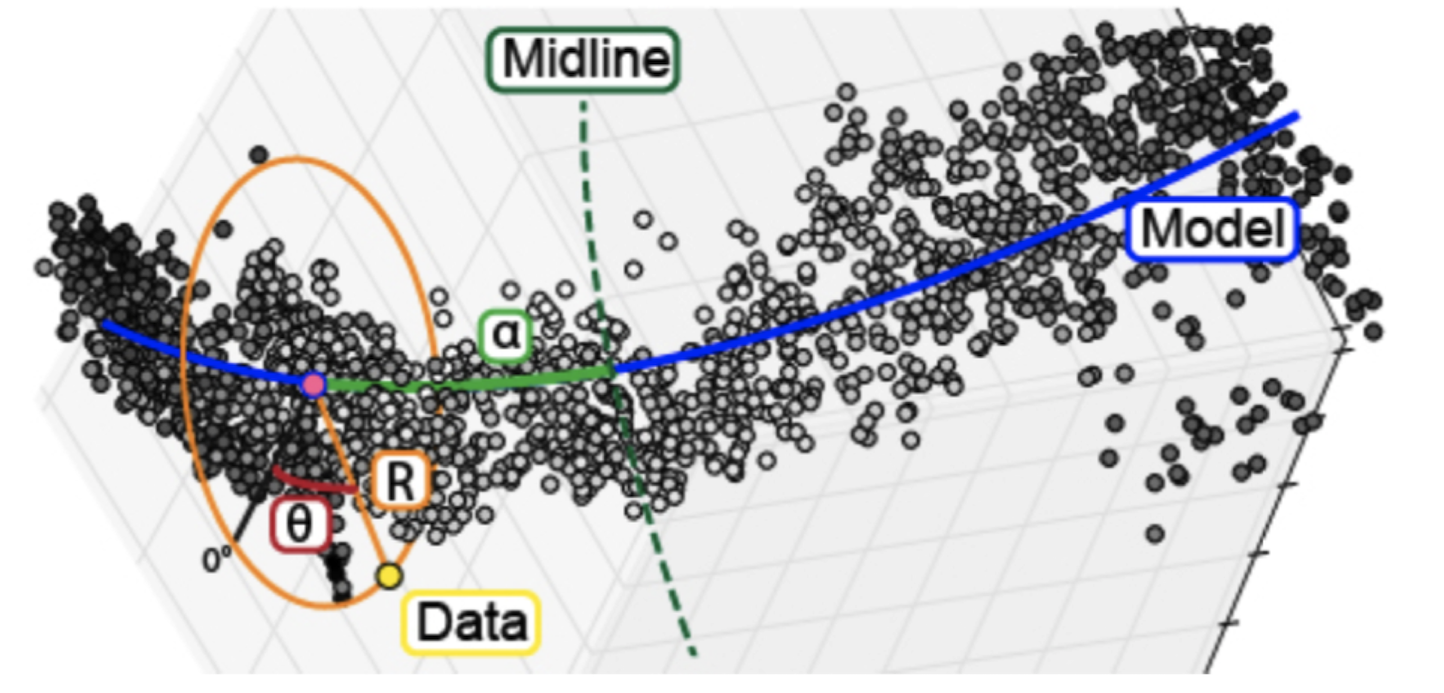
\includegraphics[width=5.55in]{figures/landmark} 

}

\caption{Landmark}\label{fig:landmark}
\end{figure}

We have 43 wildtypes samples (\(n_1\)) and 35 mutant samples (\(n_2\))
for training and testing. There are 152 landmarks (\(N\)) for each
sample, with each of them containing the following variables:

\begin{itemize}
\tightlist
\item
  number of points in each wedge
\item
  median \(r\) (micro-meter): the median of the distances to the center
  of the slice of all the points in each wedge
\item
  \(\alpha\) (micro-meter): distance from the center of the landmark to
  the midline
\item
  \(\theta\) (radian): the degree the describes the location of a wedge
  within each slice
\end{itemize}

We used the number of points and the median R to do classification via
support vector machine. For missing `median \(r\)' values due to absence
of points in particular landmarks, we filled them with the median value
of all the points in that landmark.

\subsection{Tidy Data}\label{tidy-data}

The raw landmarks data is a wide table containing the sample index and
all the columns holding information regarding the minimum and maximum
values of \(\alpha\) and \(\theta\), number of points, median r value,
and the type of sample for a particular sample in each landmark. and The
value in each cell refers to the median r value or number of points.
However, because all of such variables were joined by underscores in the
variable names, such as \texttt{-14.29\_-4.76\_-0.79\_0.0\_50\_pts} or
\texttt{-14.29\_-4.76\_-0.79\_0.0\_50\_r}, it was very difficult to see
what each column actually represented. Thus, the data set was
restructured to have the sample index, minimum and maximum \(\alpha\),
minimum and maximum \(\theta\), number of points, median \(r\), and type
of sample each be its own column.

Hence, three key functions were used from the tidyr package {[}3{]}:
gather(), separate(), and spread(). The gather() function separated the
dataset into key and value pairs for each index. The key was the column
name containing all essential information connected by underscores and
the value included the number of points or median r value. Then, the
separate() function separated the result from the gather function
divided the column connected by underscore into 5 different columns,
named as \texttt{min\_alpha}, \texttt{max\_alpha}, \texttt{min\_theta},
\texttt{max\_theta}, and \texttt{ptsOrR}. This was added to the result
of the gather function that contained the index and value of each cell,
either median R or number of points. Afterwards, the spread() function
widened the already wide table by expanding the \texttt{ptsOrR} column
by creating two columns, each column representing median R and the
number of points.

\subsection{Dealing with Missing
Values}\label{dealing-with-missing-values}

Support Vector Machine (SVM) cannot be fit to data with missing values.
For wedges that do not have any points, \texttt{median\ r} cannot be
calculated, which means that these sample will be eliminated when
running SVM. Wedges without points have biologically meanings, so we
should not ignore these wedges in our model. In order to keep the wedges
in our model, we need to artificially pick a \texttt{median\ r} value to
replace the missing ones. SVM is sensitive to outliers, so we cannot
pick an \texttt{r} value that could become outliers. We decided to
calculate the mean of \texttt{median\ r} for the nth landmark of all 78
samples, and then we replace the missing \texttt{median\ r} values with
the 2 * median R value for each landmark of each channel.

\section{Support Vector Machine}\label{support-vector-machine}

The goal of SVM is to find a separation line
\(f(x) = (\beta_0 + \beta_1 \cdot x_1 + \beta_2 \cdot x_2)\) that
separates the nearest data as cleanly as possible. The parameters
\(\beta\) are found by solving the optimization problem --to maximize M
subject to some restrictions -- in 2 dimensions below.

\begin{figure}[h]

{\centering 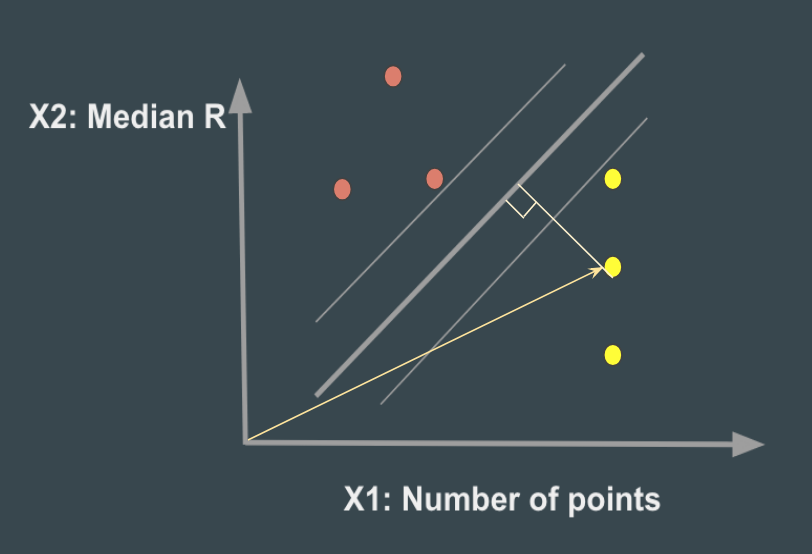
\includegraphics[width=3.12in]{figures/svm_fig} 

}

\caption{SVM model}\label{fig:svmfig}
\end{figure}

\begin{equation}
  \left.
  \begin{array}{l@{\,}l}
     \sum_{i=1}^n \beta_i^2 = 0 \\
     \ y_i * ( \beta_0 + \beta_1 \cdot x_1 + \beta_2 \cdot x_2 ) \geq M(1-\varepsilon_i) \\
     \ \varepsilon_i \geq 0 \\
     \ \sum_{i=1}^n \varepsilon_i \leq C \\
  \end{array}
  \right.
\end{equation}

\begin{itemize}
\tightlist
\item
  \(C\): tuning parameter, toleration of misclassification.
\item
  \(M\): margin is the distance of the closest points to the hyperplane.
  It is the distance between the two light grey lines.
\item
  \(\varepsilon_i\) : slack variable, an observation is classified at
  the correct/incorrect side of the margin.
\end{itemize}

The slack variable \(\varepsilon_i\) tells us where the ith observation
is located, relative to the separation line and relative to the margin.
If \(\varepsilon_i = 0\) then the ith observation is on the correct side
of the margin. If \(\varepsilon_i > 0\) then the ith observation is on
the wrong side of the margin. If \(\varepsilon_i > 1\) then it is on the
wrong side of the separation line.

The tuning parameter C bounds the sum of the \(\varepsilon_i\), and so
it determines the number and severity of the violations to the margin
and to the separation line that we will tolerate. We can think of C as a
budget for the amount that the margin can be violated by the n
observations. If \(C = 0\) then there is no budget for violations to the
margin, and it must be the case that
\(\varepsilon_1 = . . . = \varepsilon_n = 0\). For \(C > 0\) no more
than C observations can be on the wrong side of the separation line,
because if an observation is on the wrong side of the separation line
then \(\varepsilon_i > 1\). As the budget C increases, we become more
tolerant of violations to the margin, and so the margin will widen.
Conversely, as C decreases, we become less tolerant of violations to the
margin and so the margin narrows.

The function of the separation line:

\[f(x) = \beta_0 + \beta_1 \cdot x_1 + \beta_2 \cdot x_2 \] \(y_i\) is
the vector representing the coordinate of a data point. The dot product
of \(y_i\) and the function of the seperation line gives the
perpendicular distance from the data point to the separation line:

\[ y_i * ( \beta_0 + \beta_1 * x_1 + \beta_2 * x_2 )\]

If the dot product is greater than 0, the observation falls at the right
side of the separation line and vice versa.

\subsection{Cross-Validation}\label{cross-validation}

For our project, we have access to 43 wild-type samples and 35
mutant-type samples. Due to this limited sample size, we decided to use
a leave-one-out cross validation method to test our model.\\
For each testing sample, we built 152 SVMs for each landmark. For each
SVM, we used 10-fold cross validation to select a tuning parameter C
value among 0.1, 1 and 10.

\section{Final Product: Two-Step Interactive Classification
Tool}\label{final-product-two-step-interactive-classification-tool}

We created a two-step interactive classification tool which allows users
to simply input a data file and get an visualization of the modeling
result. There are two main components in the tool:

\subsection{General Workflow}\label{general-workflow}

\begin{figure}[h]

{\centering 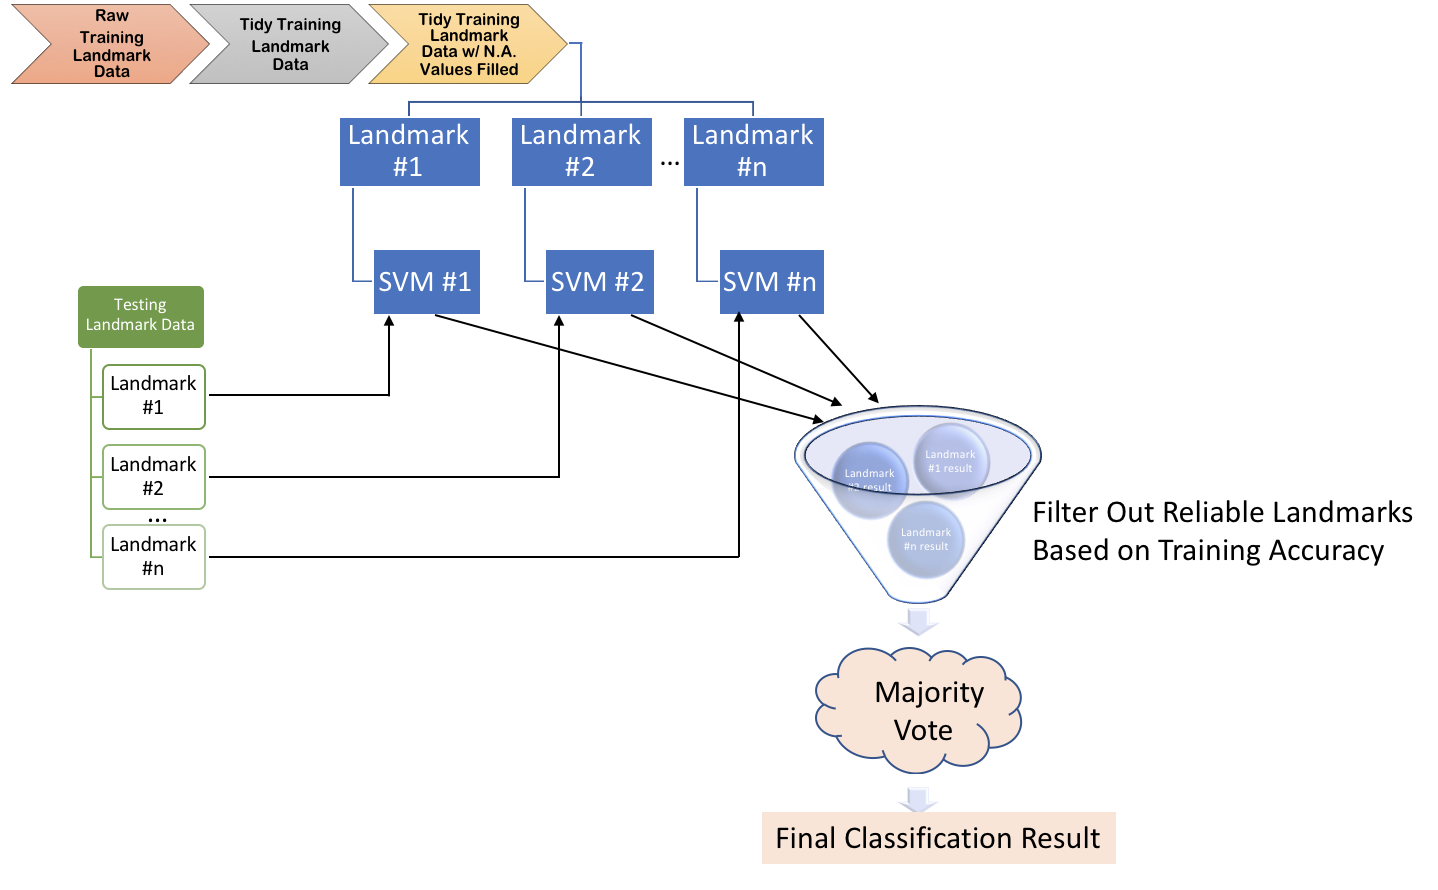
\includegraphics{figures/Figure1} 

}

\caption{Summary of Workflow}\label{fig:workflow}
\end{figure}

\textbf{Fig 2} displays the overall workflow leading to the final
product of classification. It begins with the cleaning and restructuring
of the raw landmarks data. The tidied landmarks data that has the NA
values filled contains 152 distinct landmarks. Each landmark has its own
representative SVM model that used the 77 samples out of 78 for training
from applying the leave-one-out cross validation method. That one sample
that is left out from each landmark is used for testing the model that
was built from the 77 samples. Then, based on the training accuracy of
each model, only those that consist of reliable landmarks are filtered
out. The number of wildtypes and mutants predicted with each model are
calculated and this leads to the final classification result of using
SVMs.

\subsection{Step One: Data Processing and
Modelling}\label{step-one-data-processing-and-modelling}

This step is implemented using \textbf{Python} (version 3) and packages
including \texttt{pandas}, \texttt{numpy} and \texttt{sklearn} are
required. Users would need to run and interact with the Python script
\texttt{svm.py} to pre-process the data and build the model. Then, they
would need to run another script \texttt{analyse\_results.py} to analyse
the raw results and produce aggregated results.

The script \texttt{svm.py} contains two components: a general-purpose
\texttt{svm\_classification()} function that builds a SVM model to
classify points for a perticular landmark and a \texttt{main()} function
that runs the \texttt{svm\_classification()} function for each landmark.

The script \texttt{analyse\_results.py} contains three components: a
helper function \texttt{get\_result\_file\_pathes()} that returns a list
of result file pathes in the output folder; a helper function
\texttt{process\_row\_data()} that takes a path of raw data file and
returns one with accuracy scores calculated and attached; a
\texttt{main()} function that runs the two helper function to process
all raw data files and generates an aggregated CSV file comtaining
results from all samples.

\subsubsection{User Interaction}\label{user-interaction}

\begin{figure}[h]

{\centering 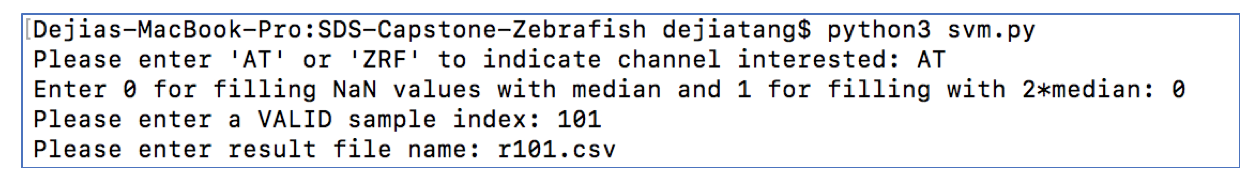
\includegraphics{figures/Figure2} 

}

\caption{Example of User Interaction in Step One of the User Interface}\label{fig:useri}
\end{figure}

\begin{figure}[h]
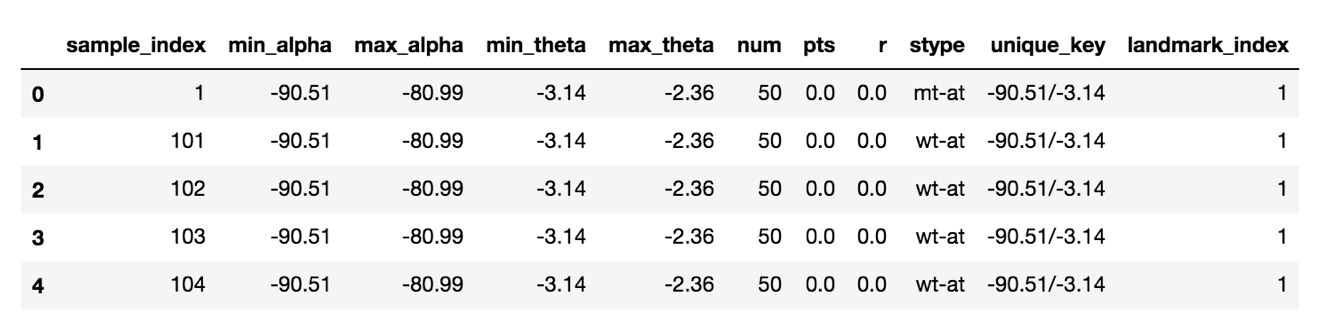
\includegraphics[width=5.11in]{figures/Figure3} \caption{Example of User Interaction for Running svm.py}\label{fig:useri2}
\end{figure}

As shown in \textbf{Fig 3} and \textbf{Fig 4}, several user inputs are
taken from users when they run the python scriptsf.

\subsubsection{Input File}\label{input-file}

Input file must contain landmark data. Variables that are needed for
classification are required to be included in the input file. In our
analysis, we used number of points in each sub-section corresponding to
each landmark of the 3D shape and the \texttt{median\ R} of points in
each wedge.

\subsubsection{Sample input file}\label{sample-input-file}

\begin{figure}[h]
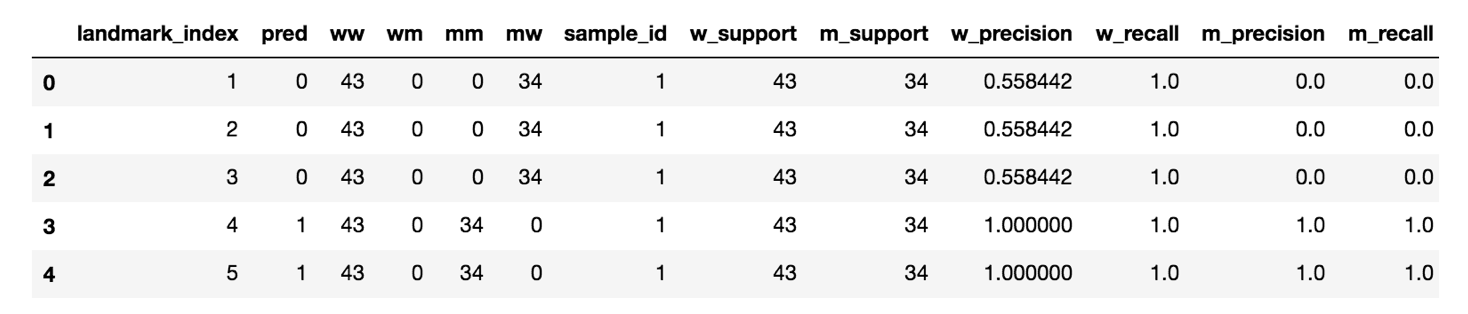
\includegraphics[width=300px]{figures/Figure4} \caption{Random Sample of a Input File for svm.py}\label{fig:inputdata}
\end{figure}

\textbf{Fig 5} shows a ramdom sample of an input file for the script
\texttt{svm.py}. The columns \texttt{stype}(sample type),
\texttt{landmark\_index} and \texttt{sample\_index} are arequired and
the other two columns (\texttt{pts} and \texttt{r} in this example) are
the two parameters for building SVM.

\subsubsection{Output File}\label{output-file}

\begin{figure}[h]

{\centering 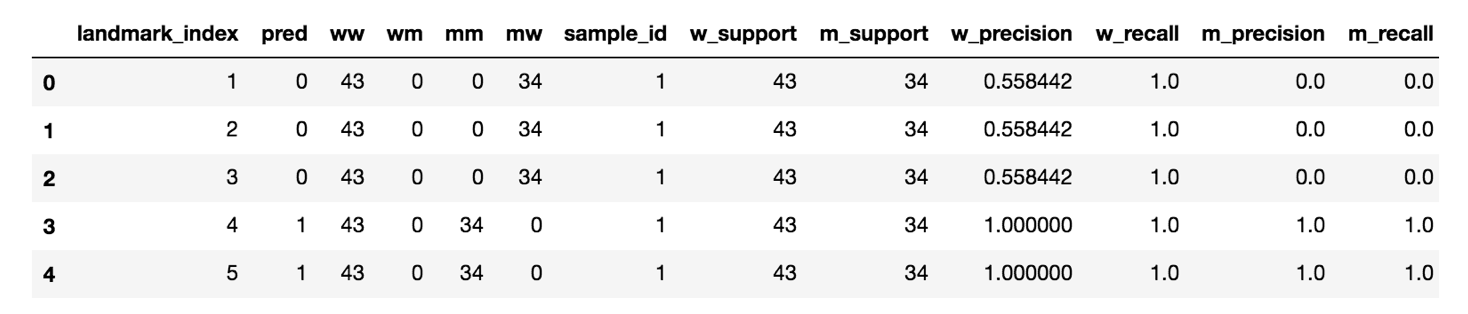
\includegraphics[width=5.65in]{figures/Figure4} 

}

\caption{Sample Data Output File of First Step of the User Interface}\label{fig:outputdata}
\end{figure}

\begin{figure}[h]
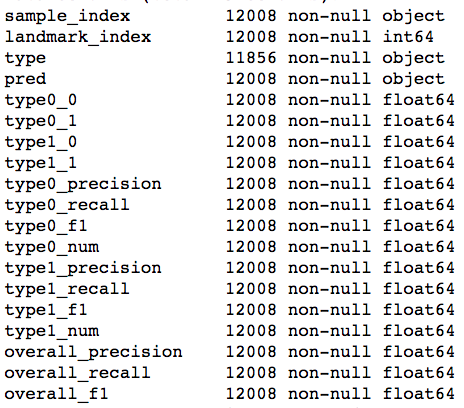
\includegraphics[width=300px]{figures/Figure5} \caption{Output File Columns of Aggregated Result}\label{fig:outputdata2}
\end{figure}

\textbf{Fig 6} shows the columns of the final result file produced by
the \texttt{analyse\_results.py} script.

\subsection{Step Two: Interactive Visualization
Tool}\label{step-two-interactive-visualization-tool}

After building SVM models in step one, we insert the output from the SVM
models into step two to visualize the results. Steps two uses the
accuracy scores output from step one to create a user-friendly app which
generates visualizations to help users to understand the SVM results.

The repository containing the shiny app can be access by doing the
following:

\begin{Shaded}
\begin{Highlighting}[]
\KeywordTok{install.packages}\NormalTok{(}\StringTok{"devtools"}\NormalTok{)}
\NormalTok{devtools::}\KeywordTok{install_github}\NormalTok{(}\StringTok{"liwencong1995/SDS-Capstone-Zebrafish"}\NormalTok{)}
\end{Highlighting}
\end{Shaded}

The file containing the source code of the shiny app can be found in
\texttt{9.FinalModel} folder of the repository. The file is named as
\texttt{shiny\_app.R}.

\subsubsection{Input 1: Data File and
Variables}\label{input-1-data-file-and-variables}

Input \texttt{CSV} data file must be stored in a folder called
\texttt{data} under your working directory, and the \texttt{CSV} file
must be named as \texttt{output\_data.csv}. If you do not know what your
working directory is, you can check it by using the function
\texttt{getwd()} in base R.

All SVM models from step one produce the following 9 accuracy
measurements:

\begin{enumerate}
\def\labelenumi{\arabic{enumi}.}
\tightlist
\item
  Precision score of type 0
\item
  Recall score of type 0
\item
  F1 score of type 0
\item
  Precision score of type 1
\item
  Recall score of type 1
\item
  F1 score of type 1
\item
  Overall precision score
\item
  Overall recall score
\item
  Overall F1 score
\end{enumerate}

These 9 accuracy scores are the variables needed in the second step of
the user interface to create the visualizations.

\subsubsection{Input 2: User Inputs}\label{input-2-user-inputs}

Users can select \texttt{channel} and \texttt{sample\ index} to filter
the input dataset to only keep the observations that users are
interested in.

In addition, users can set the threshold of the following variables:

\begin{itemize}
\tightlist
\item
  Overall precision score
\item
  Overall recall score
\item
  Overall F1 score
\end{itemize}

The dataset used to create the visualizations is rendered everytime
users cahnge one or multiple thresholds. Our app filters out the
observations that do not fulfill the threshold requirements and uses the
resulting dataset to update the histograms and heatmaps.

\subsubsection{Output: Interactive User
Interface}\label{output-interactive-user-interface}

This interactive user interface was built upon several \textbf{R}
packages:

\begin{itemize}
\tightlist
\item
  \texttt{dplyr} {[}4{]}
\item
  \texttt{data.table} {[}5{]}
\item
  \texttt{ggplot2} {[}6{]}
\item
  \texttt{shiny} {[}7{]}
\end{itemize}

We visualize the 9 accuracy scores by using both histograms and the
corresponding heatmaps that display the scores inlcuded in the
histograms in rectangular shapes that are colored with different shades
of blue according to their magnitudes. The positions of the shapes are
determined with respect to their relative positions within the
biological structure. In the study of Zebrafish, we used the relative
positions of the wedges used in landmark analysis to determine the
position of the wedges in the heatmap.

There are 10 tabs included in the user interface of the app: 1 Accuracy
Threshold Summary tab and 9 accuracy score visualization tabs.

\begin{figure}[h]

{\centering 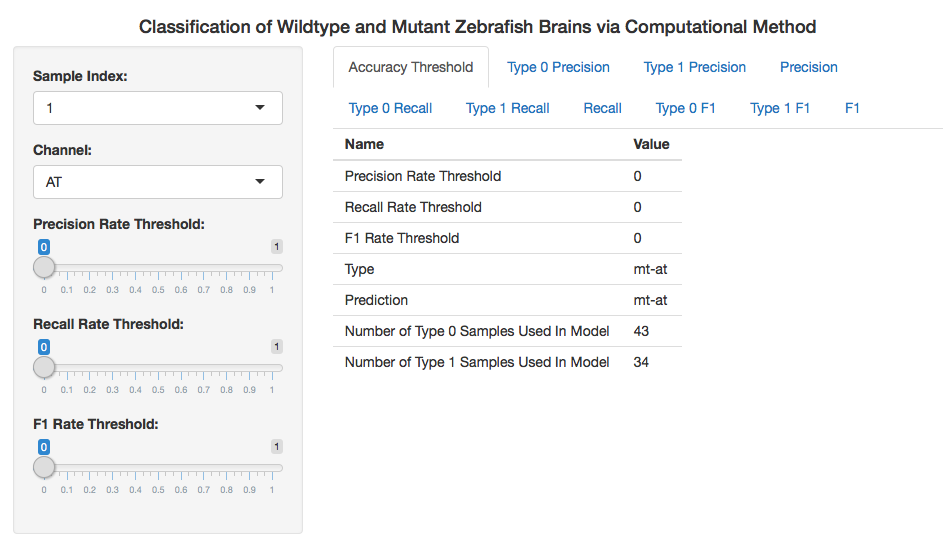
\includegraphics[width=3.66in]{figures/shiny1} 

}

\caption{User Interface: Accuracy Threshold Summary Tab of AT Channel}\label{fig:shiny1}
\end{figure}

Figure 5 displays the Accuracy Score Threshold Summary tab of the first
sample of AT channel. Users can drag the dot on the slidebar to set the
thresholds of overall precision, recall, and f1 scores. The threshold of
the three scores are updated in the summary table. Default thresholds
are 0 for all three accuracy measurements. We then use the landmark
observations that fulfill the threshold requirements to predict the type
of the sample of choice by doing a majority vote. We simply count the
total number of landmarks that are classified as type 0 and type 1, and
then we determine whether there are more of them that are classified as
type 0 or type 1. The type that gets more vote is the predicted type of
the sample. The resuting predicted sample type is also updated in the
summary table.

Other information, such as the true type of the sample and the number of
wildetypes and mutants used in training the SVM models are also included
in the summary table.

\begin{figure}[h]

{\centering 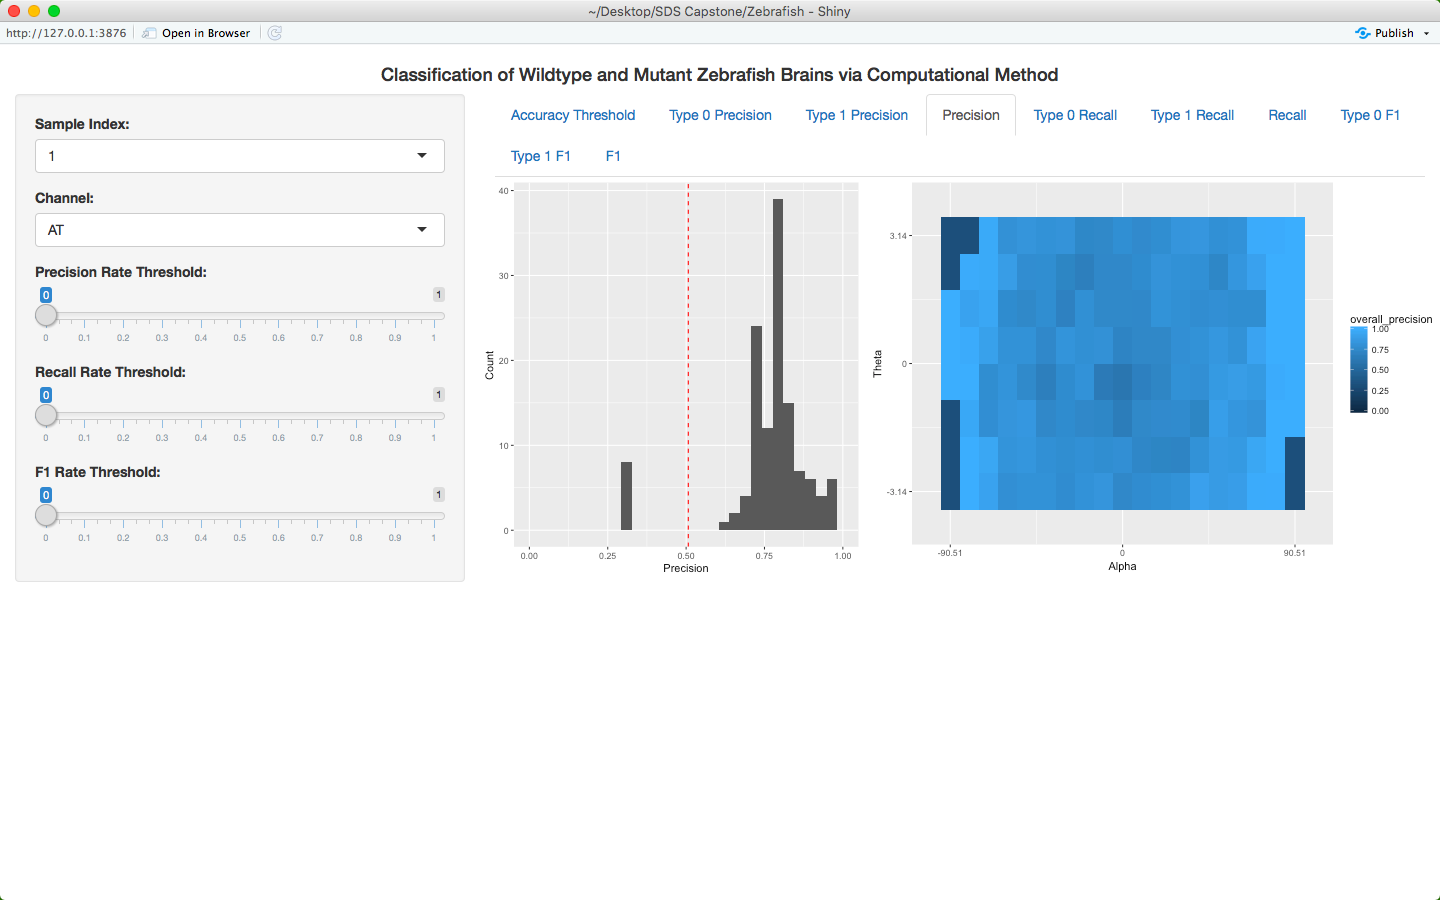
\includegraphics[width=4.92in]{figures/shiny2} 

}

\caption{User Interface: Precision Score Visualization Tab of AT Channel}\label{fig:shiny2}
\end{figure}

Figure 6 displays the Precision Score Visualization tab of the first
sample of AT channel. In this case, all three thresholds are at default
level, 0. Therefore, all landmarks' precision scores are shown in both
the histogram and the heatmap.

\begin{figure}[h]

{\centering 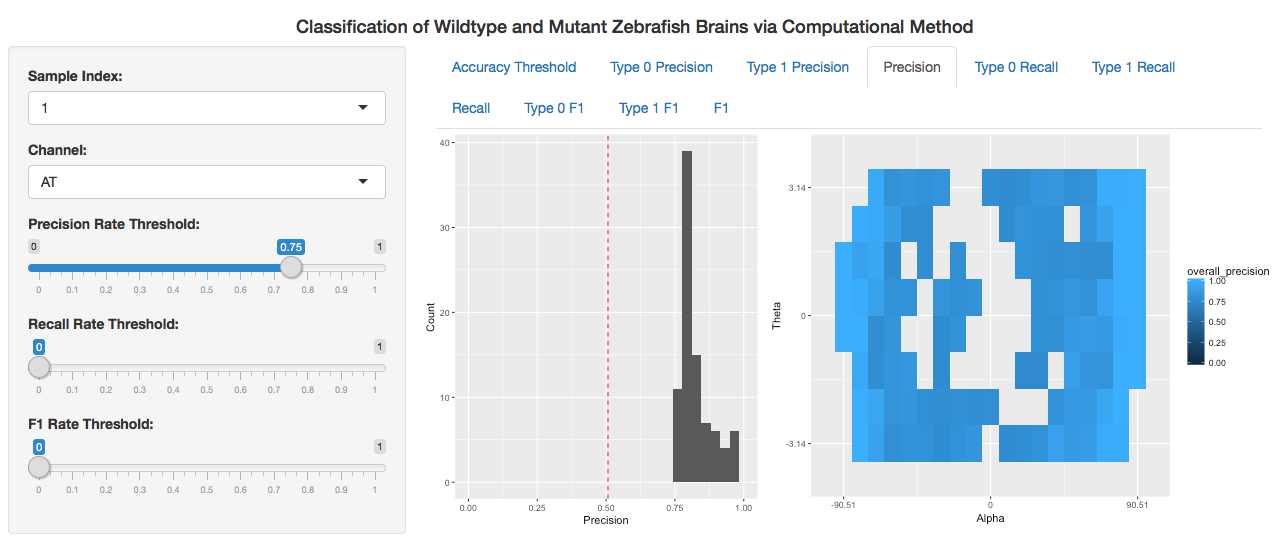
\includegraphics[width=4.9in]{figures/shiny3} 

}

\caption{User Interface: Precision Score Visualization Tab of AT Channel, with precision threshold = 0.75}\label{fig:shiny3}
\end{figure}

Figure 7 also displays the Precision Score Visualization tab of the
first sample of AT channel. In this case, recall and f1 scores'
thresholds are at default level and precision threshold is set to be
0.75. Therefore, only landmarks that have precision scores that are
equal to or greater than 0.75 are shown in the visualizations. As shown
in the histogram, all values less than 0.75 are removed from the
histogram in figure 6. Some of the blocks in figure 6 are turned into
blank blocks after the precision threshold is increased to 0.75.

\begin{figure}[h]

{\centering 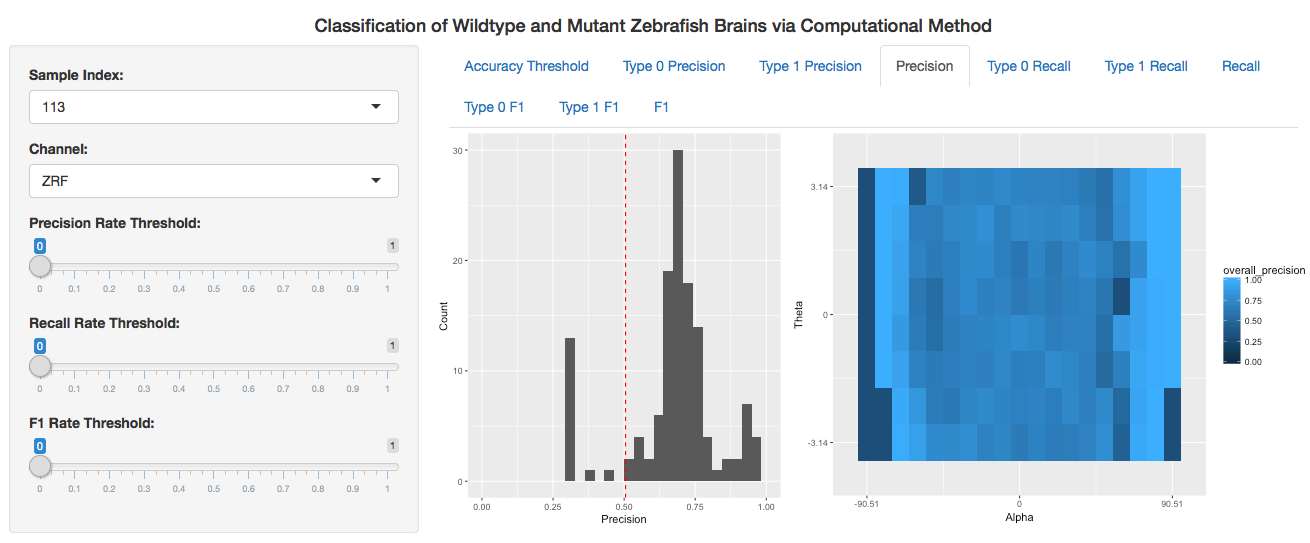
\includegraphics[width=5.04in]{figures/shiny8} 

}

\caption{User Interface: F1 Score Visualization Tab of ZRF Channel}\label{fig:shiny8}
\end{figure}

Users can also choose to observe the SVM results of ZRF channel. Figure
8 displays the Precision Score Visualization tab of the first sample of
ZRF channel with all thresholds equal to 0. More sample visualizations
of other accuracy scores can be found in Appendix A.

\section{Conclusion and Discussion}\label{conclusion-and-discussion}

\subsection{Strengths}\label{strengths}

Our final product has several strengths:

\subsubsection{Easy Interpretation}\label{easy-interpretation}

In the previous method random forest, the number of predictors \(p\)
exceeds the number of samples. Schwartz applied PCA to reduce the
dimension of the predictors. The problem with dimension reduction is
that the parameters gaining weights at last are linear combinations of
the original landmarks. While the patterns of the first several
projections still make sense, the minor projections are very random and
thus difficult to interpret.

The SVM model is generated based on landmark data gives insightful
analysis of: * which landmark, or which part of the Zebrafish brain, has
more predictive power * whether a new Zebrafish brain sample is a mutant
or wild type

\subsubsection{Implementing User
Feedback}\label{implementing-user-feedback}

We have implemented feedbacks from users in our user interface.
Originally, our shiny app only produces visualizations of one channel's
data, but we added an additional variable, \texttt{channel}, for users
to analyze three-dimentional data with more or multiple channels.
Because of this improvement, it is more convenient for users to compare
and contrast results from different channels.

\subsection{Limitations and
Improvements}\label{limitations-and-improvements}

\subsubsection{Interaction Between
Channels}\label{interaction-between-channels}

Our SVM model only make prediction of the sample type based on a single
channel's information, and it does not consider the interaction between
channels.

\subsubsection{Iterating Machine
Learning}\label{iterating-machine-learning}

Instead of cross-validation, better results could be achieved by using
iterating machine learning method. In iterative machine learning we
repeat the process of training and testing several times. At the first
round the user gives examples of objects belonging to some classes and
the machine learning algorithm is trained with this data. In the second
round, the algorithm shows examples of objects it thinks that belong to
these classes. Now, the user merely adds objects to the improved
training set which the machine learning algorithm has put into a wrong
class. That is, the user only corrects the ``misunderstandings'' of the
algorithm. In this way we can concentrate on difficult examples of
objects that are hard to classify or are for some reason easily missed
by humans. Such objects may lie close to the decision boundaries or in
the periphery in the multidimensional feature space. This iterative
process is continued until the machine learning algorithm does not make
any mistakes or the classification results do not improve anymore. It
will improve our classification results and thus is likely to help make
better predictions for unknown type.

\subsection{Future Study}\label{future-study}

\subsubsection{Interaction Between
Channels}\label{interaction-between-channels-1}

If more time is given, we could add factors that describe the
interaction between channels into our SVM model in order to combine
information from multiple channels to predict sample type.

\subsubsection{Improving User Interface}\label{improving-user-interface}

Since we have only received feedback from three users at Smith College,
we would love to get more feedbacks from other scientists and improve
our model and user interface accordingly.

\subsubsection{Improving Model Accuracy}\label{improving-model-accuracy}

\section{Acknowledgements}\label{acknowledgements}

This project was completed in partial fulfillment of the requirements of
SDS 410: SDS Capstone. This course is offered by the Statistical and
Data Sciences Program at Smith College, and was taught by Benjamin
Baumer in Spring 2018.

\newpage

\section{Appendix A: Shiny App Accuracy Score
Visualizations}\label{appendix-a-shiny-app-accuracy-score-visualizations}

\subsection{Recall Score Visualization tab of the first sample of AT
channel}\label{recall-score-visualization-tab-of-the-first-sample-of-at-channel}

\begin{figure}[h]

{\centering 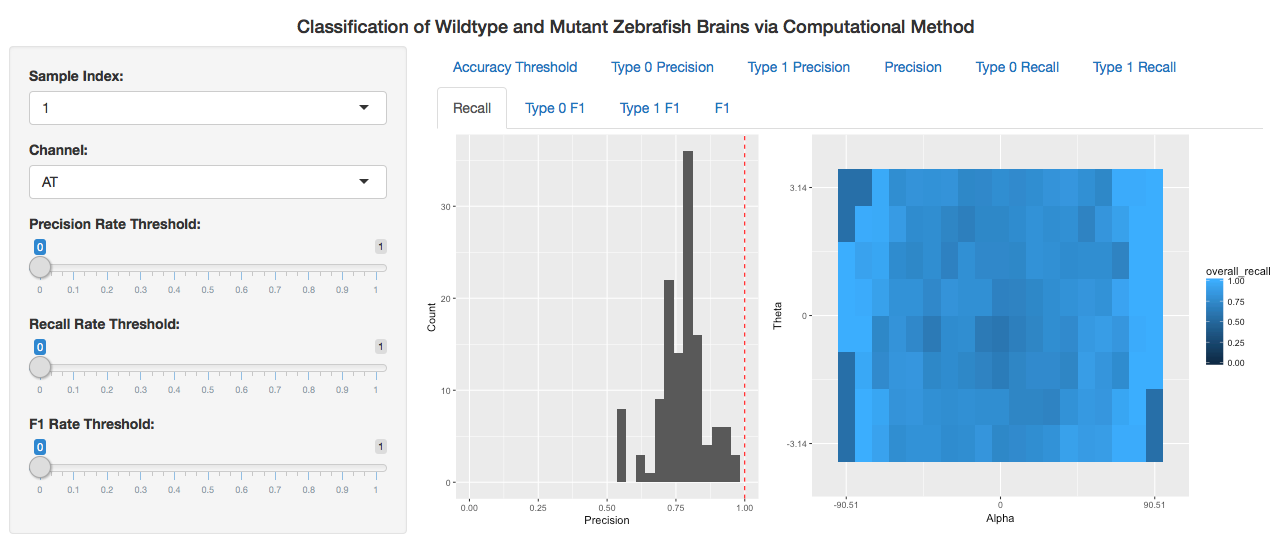
\includegraphics[width=4.91in]{figures/shiny4} 

}

\caption{User Interface: Recall Score Visualization Tab of AT Channel}\label{fig:shiny4}
\end{figure}

\subsection{Recall Score Visualization tab of the first sample of AT
channel with recall threshold equals to
0.75}\label{recall-score-visualization-tab-of-the-first-sample-of-at-channel-with-recall-threshold-equals-to-0.75}

\begin{figure}[h]

{\centering 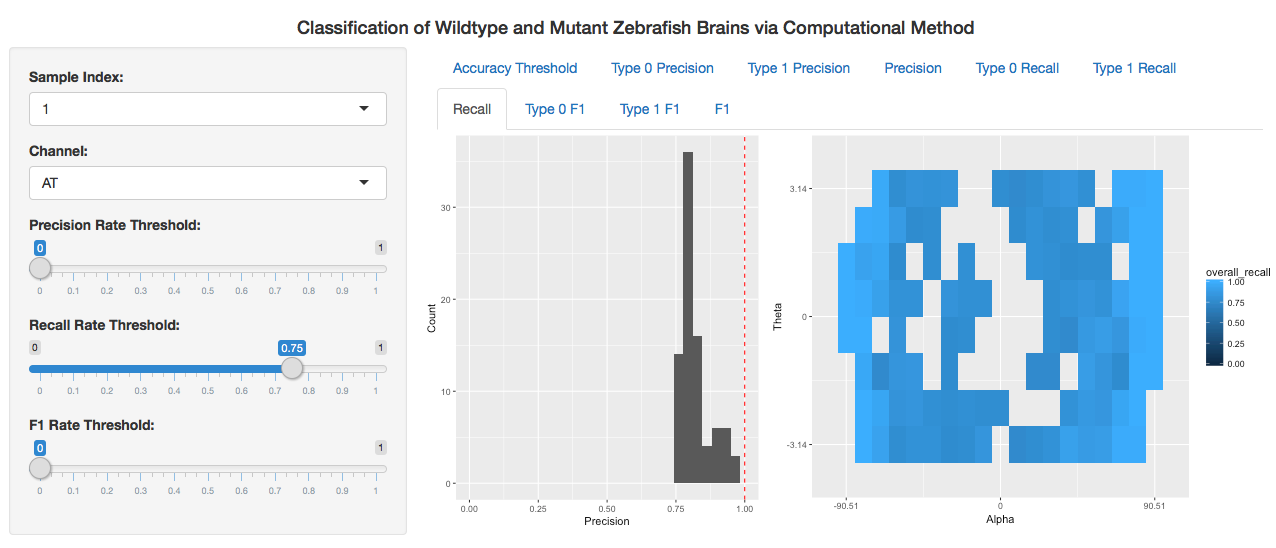
\includegraphics[width=4.91in]{figures/shiny5} 

}

\caption{User Interface: Recall Score Visualization Tab of AT Channel, with recall threshold = 0.75}\label{fig:shiny5}
\end{figure}

\newpage

\subsection{F1 Score Visualization tab of the first sample of AT
channel}\label{f1-score-visualization-tab-of-the-first-sample-of-at-channel}

\begin{figure}[h]

{\centering 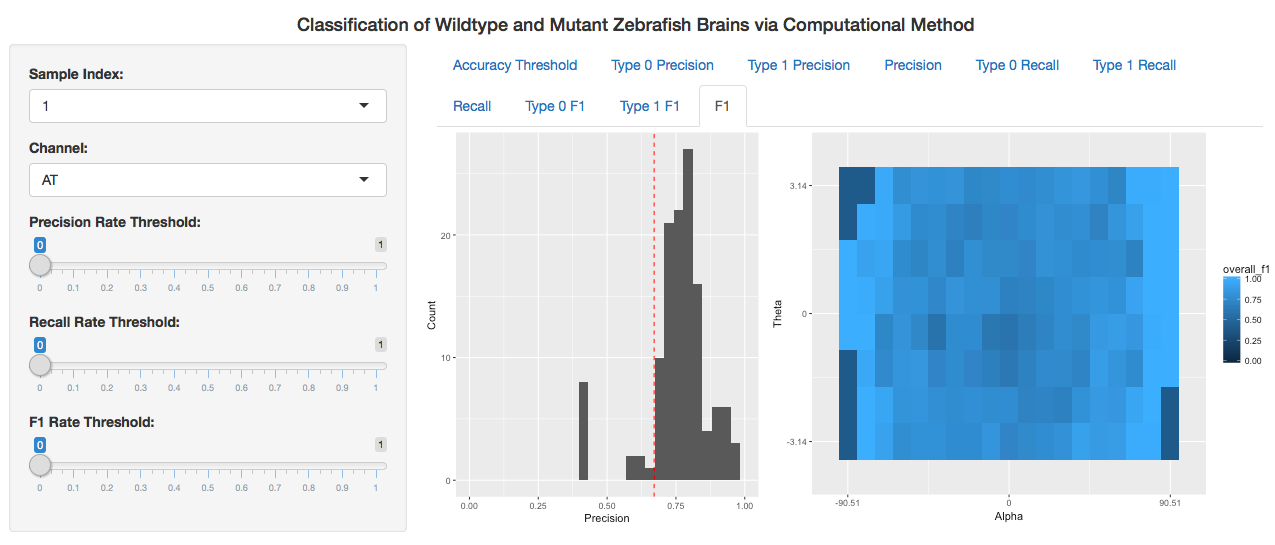
\includegraphics[width=4.9in]{figures/shiny6} 

}

\caption{User Interface: F1 Score Visualization Tab of AT Channel}\label{fig:shiny6}
\end{figure}

\subsection{F1 Score Visualization tab of the first sample of AT channel
with f1 threshold equals to
0.75}\label{f1-score-visualization-tab-of-the-first-sample-of-at-channel-with-f1-threshold-equals-to-0.75}

\begin{figure}[h]

{\centering 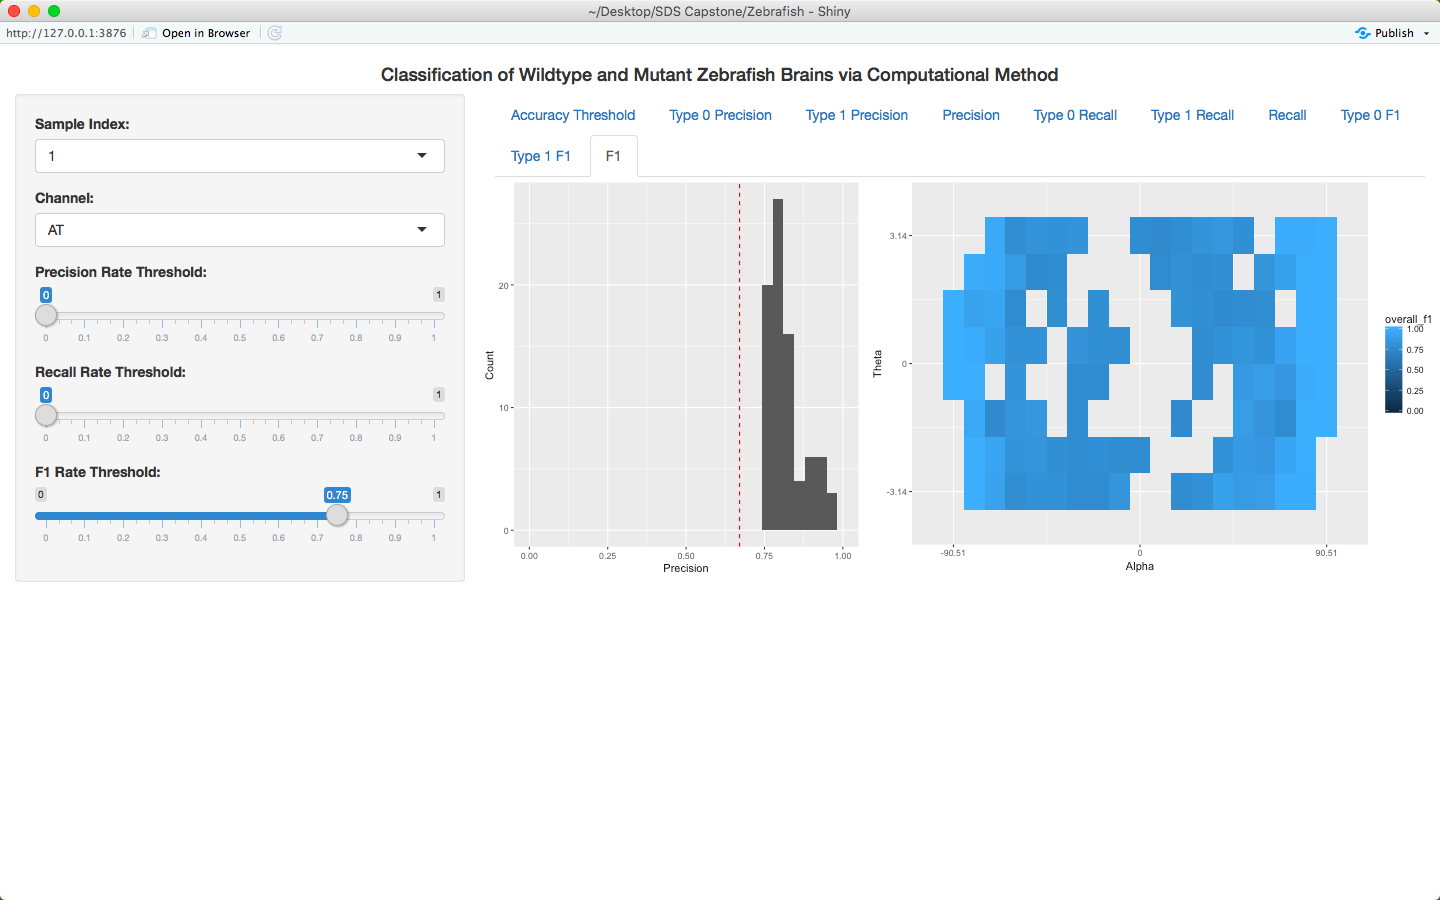
\includegraphics[width=4.9in]{figures/shiny7} 

}

\caption{User Interface: F1 Score Visualization Tab of AT Channel, with f1 threshold = 0.75}\label{fig:shiny7}
\end{figure}

\newpage

\section{Appendix B: Source Code for User
Interface}\label{appendix-b-source-code-for-user-interface}

\subsection{Support Vector Machine}\label{support-vector-machine-1}

\begin{Shaded}
\begin{Highlighting}[]
\ImportTok{import} \NormalTok{pandas }\ImportTok{as} \NormalTok{pd}
\ImportTok{import} \NormalTok{numpy }\ImportTok{as} \NormalTok{np}
\ImportTok{from} \NormalTok{sklearn.metrics }\ImportTok{import} \NormalTok{confusion_matrix, classification_report}
\ImportTok{from} \NormalTok{sklearn.model_selection }\ImportTok{import} \NormalTok{GridSearchCV}
\ImportTok{from} \NormalTok{sklearn.svm }\ImportTok{import} \NormalTok{SVC}
\ImportTok{from} \NormalTok{sklearn.metrics }\ImportTok{import} \NormalTok{f1_score, precision_score, recall_score}
\CommentTok{'''}
\CommentTok{A function that builds a SVM model with linear kernel to classify points to two classes.}
\CommentTok{Inputs:}
\CommentTok{training_landmarks - a pandas dataframe containing all training landmark data.}
\CommentTok{index              - a perticular landmark id of interest. eg. '101'}
\CommentTok{x_names            - a list of explanatory variable names. eg. ['pts', 'r']}
\CommentTok{y_name             - a string representing response variable name. eg. 'stype'}
\CommentTok{class0             - name of the first class. eg. 'wt-at'}
\CommentTok{class1             - name of the second class. eg. 'mt-at'}
\CommentTok{C_values           - a list of tunning variable C (penalty parameter of the error term) that the method would grid-search on. Default value is [0.1, 1, 10].}
\CommentTok{Output:}
\CommentTok{svm                - the SVM model trained from the training dataset}
\CommentTok{ww                 - among the training samples, the number of wild type samples with chosen landmark predicted as wild type.}
\CommentTok{wm                 - among the training samples, the number of wild type samples with chosen landmark predicted as mutant type.}
\CommentTok{mm                 - among the training samples, the number of mutant type samples with chosen landmark predicted as mutant type.}
\CommentTok{mw                 - among the training samples, the number of mutant type samples with chosen landmark predicted as wild type.}
\CommentTok{'''}
\KeywordTok{def} \NormalTok{svm_classification(training_landmarks, index, x_names, y_name, class0, class1, C_values }\OperatorTok{=} \NormalTok{[}\FloatTok{0.1}\NormalTok{, }\DecValTok{1}\NormalTok{, }\DecValTok{10}\NormalTok{] ):}
    \CommentTok{# filter out the landmarks needed}
    \NormalTok{chosenLandmark }\OperatorTok{=} \NormalTok{landmarks[landmarks.landmark_index}\OperatorTok{==}\NormalTok{index]}
    \NormalTok{chosenLandmark }\OperatorTok{=} \NormalTok{chosenLandmark[np.isfinite(chosenLandmark[}\StringTok{'r'}\NormalTok{])]}
    
    \CommentTok{# create training and testing data}
    \NormalTok{X }\OperatorTok{=} \NormalTok{chosenLandmark[x_names]}
    \NormalTok{y }\OperatorTok{=} \NormalTok{chosenLandmark[y_name]}
    \NormalTok{y }\OperatorTok{=} \NormalTok{y.replace([class1], }\DecValTok{1}\NormalTok{)}
    \NormalTok{y }\OperatorTok{=} \NormalTok{y.replace([class0], }\DecValTok{0}\NormalTok{)}
    \CommentTok{# check whether both classes exist}
    \NormalTok{count_1 }\OperatorTok{=} \NormalTok{chosenLandmark[y_name].}\BuiltInTok{str}\NormalTok{.contains(class1).}\BuiltInTok{sum}\NormalTok{()}
    \NormalTok{count_0 }\OperatorTok{=} \NormalTok{chosenLandmark[y_name].}\BuiltInTok{str}\NormalTok{.contains(class0).}\BuiltInTok{sum}\NormalTok{()}
    \ControlFlowTok{if} \NormalTok{(count_1 }\OperatorTok{<} \DecValTok{2} \OperatorTok{or} \NormalTok{count_0 }\OperatorTok{<} \DecValTok{2}\NormalTok{):}
        \ControlFlowTok{return} \VariableTok{None}\NormalTok{, }\VariableTok{None}\NormalTok{, }\VariableTok{None}\NormalTok{, }\VariableTok{None}\NormalTok{, }\VariableTok{None}
    \CommentTok{# find the best C value by cross-validation}
    \NormalTok{tuned_parameters }\OperatorTok{=} \NormalTok{[\{}\StringTok{'C'}\NormalTok{: C_values\}]}
    \NormalTok{clf }\OperatorTok{=} \NormalTok{GridSearchCV(SVC(kernel}\OperatorTok{=}\StringTok{'linear'}\NormalTok{), tuned_parameters, cv}\OperatorTok{=}\DecValTok{10}\NormalTok{, scoring}\OperatorTok{=}\StringTok{'accuracy'}\NormalTok{)}
    \NormalTok{clf.fit(X.values, y.values)}
    \NormalTok{best_c }\OperatorTok{=} \NormalTok{clf.best_params_[}\StringTok{'C'}\NormalTok{]}
    
    \NormalTok{svc }\OperatorTok{=} \NormalTok{SVC(C}\OperatorTok{=}\NormalTok{best_c, kernel}\OperatorTok{=}\StringTok{'linear'}\NormalTok{)}
    \NormalTok{svc.fit(X, y)}
    
    \NormalTok{prediction }\OperatorTok{=} \NormalTok{svc.predict(X)}
    \CommentTok{# print confusion matrix}
    \BuiltInTok{print}\NormalTok{(}\StringTok{"confusion matrix: "}\NormalTok{)}
    \NormalTok{cm }\OperatorTok{=} \NormalTok{confusion_matrix(y, prediction)}
    \NormalTok{cm_df }\OperatorTok{=} \NormalTok{pd.DataFrame(cm.T, index}\OperatorTok{=}\NormalTok{svc.classes_, columns}\OperatorTok{=}\NormalTok{svc.classes_)}
    \BuiltInTok{print}\NormalTok{(cm_df)}
    \CommentTok{# Statistics of training precision:}
    \CommentTok{# number of wild type samples with this landmark predicted as wild type.}
    \NormalTok{ww }\OperatorTok{=}\DecValTok{0}
    \CommentTok{# number of wild type samples with this landmark predicted as mutant type.}
    \NormalTok{wm }\OperatorTok{=} \DecValTok{0}
    \CommentTok{# number of mutant type samples with this landmark predicted as mutant type.}
    \NormalTok{mm }\OperatorTok{=} \DecValTok{0}
    \CommentTok{# number of mutant type samples with this landmark predicted as wild type.}
    \NormalTok{mw }\OperatorTok{=} \DecValTok{0}
    
    \ControlFlowTok{for} \NormalTok{i }\OperatorTok{in} \BuiltInTok{range} \NormalTok{(}\BuiltInTok{len}\NormalTok{(y)):}
        \NormalTok{_y }\OperatorTok{=} \NormalTok{y.values[i]}
        \NormalTok{_p }\OperatorTok{=} \NormalTok{prediction[i]}
        \ControlFlowTok{if} \NormalTok{_y}\OperatorTok{==}\DecValTok{1} \OperatorTok{and} \NormalTok{_p}\OperatorTok{==}\DecValTok{1}\NormalTok{:}
            \NormalTok{mm }\OperatorTok{=} \NormalTok{mm }\OperatorTok{+} \DecValTok{1}
        \ControlFlowTok{elif} \NormalTok{_y}\OperatorTok{==}\DecValTok{1} \OperatorTok{and} \NormalTok{_p}\OperatorTok{==}\DecValTok{0}\NormalTok{:}
            \NormalTok{mw }\OperatorTok{=} \NormalTok{mw }\OperatorTok{+} \DecValTok{1}
        \ControlFlowTok{elif} \NormalTok{_y}\OperatorTok{==}\DecValTok{0} \OperatorTok{and} \NormalTok{_p}\OperatorTok{==}\DecValTok{0}\NormalTok{:}
            \NormalTok{ww }\OperatorTok{=} \NormalTok{ww }\OperatorTok{+} \DecValTok{1}
        \ControlFlowTok{elif} \NormalTok{_y}\OperatorTok{==}\DecValTok{0} \OperatorTok{and} \NormalTok{_p}\OperatorTok{==}\DecValTok{1}\NormalTok{:}
            \NormalTok{wm }\OperatorTok{=} \NormalTok{wm }\OperatorTok{+} \DecValTok{1}
    
    \ControlFlowTok{return} \NormalTok{svc, ww, wm, mm, mw}
\ControlFlowTok{if} \VariableTok{__name__} \OperatorTok{==} \StringTok{"__main__"}\NormalTok{:}
    \CommentTok{# Get interested chnnel name}
    \NormalTok{channel }\OperatorTok{=} \StringTok{''}
    \ControlFlowTok{while} \NormalTok{(channel }\OperatorTok{!=} \StringTok{'AT'} \OperatorTok{and} \NormalTok{channel }\OperatorTok{!=} \StringTok{'ZRF'}\NormalTok{):}
        \NormalTok{channel }\OperatorTok{=} \BuiltInTok{input}\NormalTok{(}\StringTok{"Please enter 'AT' or 'ZRF' to indicate channel interested: "}\NormalTok{)}
    
    \NormalTok{class0 }\OperatorTok{=} \StringTok{'mt-zrf'} \ControlFlowTok{if} \NormalTok{channel }\OperatorTok{==} \StringTok{'ZRF'} \ControlFlowTok{else} \StringTok{'mt-at'}
    \NormalTok{class1 }\OperatorTok{=} \StringTok{'wt-zrf'} \ControlFlowTok{if} \NormalTok{channel }\OperatorTok{==} \StringTok{'ZRF'} \ControlFlowTok{else} \StringTok{'wt-at'}
    \CommentTok{# Read in landmark data}
    \NormalTok{data_type }\OperatorTok{=} \StringTok{'-1'}
    \ControlFlowTok{while} \NormalTok{(data_type }\OperatorTok{!=} \StringTok{'0'} \OperatorTok{and} \NormalTok{data_type }\OperatorTok{!=} \StringTok{'1'}\NormalTok{):}
        \NormalTok{data_type }\OperatorTok{=} \BuiltInTok{input}\NormalTok{(}\StringTok{"Enter 0 for filling NaN values with median and 1 for filling with 2*median: "}\NormalTok{)}
    \NormalTok{landmarks }\OperatorTok{=} \NormalTok{pd.DataFrame()}
    \ControlFlowTok{if} \NormalTok{(channel }\OperatorTok{==} \StringTok{'AT'}\NormalTok{):}
        \NormalTok{landmarks }\OperatorTok{=} \NormalTok{pd.read_csv(}\StringTok{'./data/final/landmark_AT_filled_w_median.csv'}\NormalTok{) }\ControlFlowTok{if} \NormalTok{data_type}\OperatorTok{==}\StringTok{'0'} \ControlFlowTok{else} \NormalTok{pd.read_csv(}\StringTok{'./data/final/landmark_AT_filled_w_2median.csv'}\NormalTok{)}
    \ControlFlowTok{else}\NormalTok{:}
        \NormalTok{landmarks }\OperatorTok{=} \NormalTok{pd.read_csv(}\StringTok{'./data/final/landmark_ZRF_filled_w_median.csv'}\NormalTok{) }\ControlFlowTok{if} \NormalTok{data_type}\OperatorTok{==}\StringTok{'0'} \ControlFlowTok{else} \NormalTok{pd.read_csv(}\StringTok{'./data/final/landmark_ZRF_filled_w_2median.csv'}\NormalTok{)}
    \CommentTok{# Get sample id}
    \NormalTok{sample }\OperatorTok{=} \NormalTok{pd.DataFrame()}
    \ControlFlowTok{while}\NormalTok{(sample.shape[}\DecValTok{0}\NormalTok{]}\OperatorTok{<}\DecValTok{2}\NormalTok{):}
        \NormalTok{sample_id }\OperatorTok{=} \BuiltInTok{str}\NormalTok{(}\BuiltInTok{input}\NormalTok{(}\StringTok{"Please enter a VALID sample index: "}\NormalTok{))}
        \NormalTok{sample }\OperatorTok{=} \NormalTok{landmarks[landmarks.sample_index}\OperatorTok{==}\NormalTok{sample_id]}
    \CommentTok{# Get result file's name and create the file with column names}
    \NormalTok{result_file_name }\OperatorTok{=} \BuiltInTok{str}\NormalTok{(}\BuiltInTok{input}\NormalTok{(}\StringTok{"Please enter result file name: "}\NormalTok{))}
    \NormalTok{result_file }\OperatorTok{=} \BuiltInTok{open}\NormalTok{(result_file_name, }\StringTok{'w'}\NormalTok{)}
    \NormalTok{result_file.write(}\StringTok{'sample_index, landmark_index, pred, ww, wm, mm, mw}\CharTok{\textbackslash{}n}\StringTok{'}\NormalTok{)}
    \NormalTok{result_file.close()}
    \CommentTok{# Get existing landmark ids}
    \NormalTok{landmark_ids }\OperatorTok{=} \NormalTok{sample[}\StringTok{'landmark_index'}\NormalTok{]}
    \NormalTok{leave_one_out }\OperatorTok{=} \NormalTok{landmarks[landmarks.sample_index}\OperatorTok{!=}\NormalTok{sample_id]}
    \ControlFlowTok{for} \NormalTok{l }\OperatorTok{in} \NormalTok{landmark_ids.values:}
        \BuiltInTok{print} \NormalTok{(}\StringTok{"======================================="}\NormalTok{)}
        \BuiltInTok{print} \NormalTok{(}\StringTok{"landmark: "}\NormalTok{, }\BuiltInTok{str}\NormalTok{(l))}
        \NormalTok{svc, ww, wm, mm, mw }\OperatorTok{=} \NormalTok{svm_classification(training_landmarks }\OperatorTok{=} \NormalTok{leave_one_out,}
                                                 \NormalTok{index }\OperatorTok{=} \NormalTok{l,}
                                                 \NormalTok{x_names }\OperatorTok{=} \NormalTok{[}\StringTok{'pts'}\NormalTok{, }\StringTok{'r'}\NormalTok{],}
                                                 \NormalTok{y_name }\OperatorTok{=} \StringTok{'stype'}\NormalTok{,}
                                                 \NormalTok{class0 }\OperatorTok{=} \NormalTok{class0,}
                                                 \NormalTok{class1 }\OperatorTok{=} \NormalTok{class1,}
                                                 \NormalTok{C_values }\OperatorTok{=} \NormalTok{[}\FloatTok{0.1}\NormalTok{, }\DecValTok{1}\NormalTok{, }\DecValTok{10}\NormalTok{])}
        \ControlFlowTok{if} \NormalTok{(svc }\OperatorTok{is} \VariableTok{None}\NormalTok{):}
            \BuiltInTok{print}\NormalTok{(}\StringTok{"One of the classes have too few samples for this landmark, so skipping it."}\NormalTok{)}
            \ControlFlowTok{continue}
        \NormalTok{prediction }\OperatorTok{=} \NormalTok{svc.predict(sample[sample.landmark_index}\OperatorTok{==}\NormalTok{l][[}\StringTok{'pts'}\NormalTok{, }\StringTok{'r'}\NormalTok{]])}
        \NormalTok{result }\OperatorTok{=} \StringTok{', '}\NormalTok{.join(}\BuiltInTok{str}\NormalTok{(x) }\ControlFlowTok{for} \NormalTok{x }\OperatorTok{in} \NormalTok{[sample_id, l, prediction[}\DecValTok{0}\NormalTok{], ww, wm, mm, mw]) }\OperatorTok{+} \StringTok{'}\CharTok{\textbackslash{}n}\StringTok{'}
        \BuiltInTok{print}\NormalTok{(}\StringTok{'result:'}\NormalTok{, result)}
        \NormalTok{result_file }\OperatorTok{=} \BuiltInTok{open}\NormalTok{(result_file_name, }\StringTok{'a'}\NormalTok{)}
        \NormalTok{result_file.write(result)}
        \NormalTok{result_file.close()}
\end{Highlighting}
\end{Shaded}

\subsection{Shiny App}\label{shiny-app}

\subsubsection{Package Dependency}\label{package-dependency}

\begin{Shaded}
\begin{Highlighting}[]
\CommentTok{# Shiny App---------------------------------------------------}
\CommentTok{# Loading packages needed in the creation of the Shiny App}
\KeywordTok{library}\NormalTok{(dplyr)}
\KeywordTok{library}\NormalTok{(data.table)}
\KeywordTok{library}\NormalTok{(ggplot2)}
\KeywordTok{library}\NormalTok{(shiny)}
\end{Highlighting}
\end{Shaded}

\subsubsection{User Input}\label{user-input}

\begin{Shaded}
\begin{Highlighting}[]
\CommentTok{# User Input -------------------------------------------------}
\CommentTok{# Please modify the file directory accordingly}
\NormalTok{data <-}\StringTok{ }\KeywordTok{fread}\NormalTok{(}\StringTok{"data/output_data_type0.csv"}\NormalTok{)}

\CommentTok{# List of input variables ------------------------------------}
\NormalTok{list_of_indices <-}\StringTok{ }\KeywordTok{c}\NormalTok{(}\KeywordTok{unique}\NormalTok{(data$sample_index)) }
\CommentTok{# Please add or subtract channels from the list_of_channels accordingly}
\NormalTok{list_of_channels <-}\StringTok{ }\KeywordTok{c}\NormalTok{(}\StringTok{"type0"}\NormalTok{, }\StringTok{"type1"}\NormalTok{)}
\end{Highlighting}
\end{Shaded}

\subsubsection{User Interface}\label{user-interface}

\begin{Shaded}
\begin{Highlighting}[]
\CommentTok{# User Interface}
\NormalTok{ui <-}\StringTok{ }\KeywordTok{fluidPage}\NormalTok{(}
  \KeywordTok{titlePanel}\NormalTok{(}\DataTypeTok{title=}\KeywordTok{h4}\NormalTok{(}\StringTok{"Classification of Wildtype and Mutant }
\StringTok{                      Zebrafish Brains via Computational Method"}\NormalTok{, }
                      \DataTypeTok{align=}\StringTok{"center"}\NormalTok{)),}
  
  \CommentTok{# Sidebar containing all input variables}
  \KeywordTok{sidebarLayout}\NormalTok{(}
    
    \CommentTok{# User Inputs}
    \KeywordTok{sidebarPanel}\NormalTok{(}
      \KeywordTok{selectInput}\NormalTok{(}\StringTok{"sampleindex"}\NormalTok{, }\StringTok{"Sample Index:"}\NormalTok{, list_of_indices),}
      \KeywordTok{selectInput}\NormalTok{(}\StringTok{"channel"}\NormalTok{, }\StringTok{"Channel:"}\NormalTok{, list_of_channels),}
      
      \CommentTok{# Input accuracy score threshold: 0-1 intervals}
      \KeywordTok{sliderInput}\NormalTok{(}\StringTok{"precision"}\NormalTok{, }\StringTok{"Precision Rate Threshold:"}\NormalTok{,}
                  \DataTypeTok{min =} \DecValTok{0}\NormalTok{, }\DataTypeTok{max =} \DecValTok{1}\NormalTok{,}
                  \DataTypeTok{value =} \DecValTok{0}\NormalTok{, }\DataTypeTok{step =} \FloatTok{0.01}\NormalTok{),}
      \KeywordTok{sliderInput}\NormalTok{(}\StringTok{"recall"}\NormalTok{, }\StringTok{"Recall Rate Threshold:"}\NormalTok{,}
                  \DataTypeTok{min =} \DecValTok{0}\NormalTok{, }\DataTypeTok{max =} \DecValTok{1}\NormalTok{,}
                  \DataTypeTok{value =} \DecValTok{0}\NormalTok{, }\DataTypeTok{step =} \FloatTok{0.01}\NormalTok{),}
      \KeywordTok{sliderInput}\NormalTok{(}\StringTok{"f1"}\NormalTok{, }\StringTok{"F1 Rate Threshold:"}\NormalTok{,}
                  \DataTypeTok{min =} \DecValTok{0}\NormalTok{, }\DataTypeTok{max =} \DecValTok{1}\NormalTok{,}
                  \DataTypeTok{value =} \DecValTok{0}\NormalTok{, }\DataTypeTok{step =} \FloatTok{0.01}\NormalTok{)}
    \NormalTok{),}
    
    \CommentTok{# Output}
    \KeywordTok{mainPanel}\NormalTok{(}
      \KeywordTok{tabsetPanel}\NormalTok{(}
        \KeywordTok{tabPanel}\NormalTok{(}\StringTok{"Accuracy Threshold"}\NormalTok{,}\KeywordTok{tableOutput}\NormalTok{(}\StringTok{"values"}\NormalTok{)),}
        \CommentTok{#heatmaps and histograms, side by side}
        \KeywordTok{tabPanel}\NormalTok{(}\StringTok{"Type 0 Precision"}\NormalTok{, }\KeywordTok{fluidRow}\NormalTok{(}
          \KeywordTok{splitLayout}\NormalTok{(}\DataTypeTok{cellWidths =} \KeywordTok{c}\NormalTok{(}\StringTok{"40%"}\NormalTok{, }\StringTok{"60%"}\NormalTok{), }
                      \KeywordTok{plotOutput}\NormalTok{(}\StringTok{"plot2"}\NormalTok{), }\KeywordTok{plotOutput}\NormalTok{(}\StringTok{"plot1"}\NormalTok{))}
          \NormalTok{)), }
        \KeywordTok{tabPanel}\NormalTok{(}\StringTok{"Type 1 Precision"}\NormalTok{, }\KeywordTok{fluidRow}\NormalTok{(}
          \KeywordTok{splitLayout}\NormalTok{(}\DataTypeTok{cellWidths =} \KeywordTok{c}\NormalTok{(}\StringTok{"40%"}\NormalTok{, }\StringTok{"60%"}\NormalTok{), }
                      \KeywordTok{plotOutput}\NormalTok{(}\StringTok{"plot4"}\NormalTok{), }\KeywordTok{plotOutput}\NormalTok{(}\StringTok{"plot3"}\NormalTok{))}
          \NormalTok{)),}
        \KeywordTok{tabPanel}\NormalTok{(}\StringTok{"Precision"}\NormalTok{,}\KeywordTok{fluidRow}\NormalTok{(}
          \KeywordTok{splitLayout}\NormalTok{(}\DataTypeTok{cellWidths =} \KeywordTok{c}\NormalTok{(}\StringTok{"40%"}\NormalTok{, }\StringTok{"60%"}\NormalTok{), }
                      \KeywordTok{plotOutput}\NormalTok{(}\StringTok{"plot6"}\NormalTok{), }\KeywordTok{plotOutput}\NormalTok{(}\StringTok{"plot5"}\NormalTok{))}
          \NormalTok{)),}
        \KeywordTok{tabPanel}\NormalTok{(}\StringTok{"Type 0 Recall"}\NormalTok{, }\KeywordTok{fluidRow}\NormalTok{(}
          \KeywordTok{splitLayout}\NormalTok{(}\DataTypeTok{cellWidths =} \KeywordTok{c}\NormalTok{(}\StringTok{"40%"}\NormalTok{, }\StringTok{"60%"}\NormalTok{), }
                      \KeywordTok{plotOutput}\NormalTok{(}\StringTok{"plot8"}\NormalTok{), }\KeywordTok{plotOutput}\NormalTok{(}\StringTok{"plot7"}\NormalTok{))}
        \NormalTok{)), }
        \KeywordTok{tabPanel}\NormalTok{(}\StringTok{"Type 1 Recall"}\NormalTok{, }\KeywordTok{fluidRow}\NormalTok{(}
          \KeywordTok{splitLayout}\NormalTok{(}\DataTypeTok{cellWidths =} \KeywordTok{c}\NormalTok{(}\StringTok{"40%"}\NormalTok{, }\StringTok{"60%"}\NormalTok{), }
                      \KeywordTok{plotOutput}\NormalTok{(}\StringTok{"plot10"}\NormalTok{), }\KeywordTok{plotOutput}\NormalTok{(}\StringTok{"plot9"}\NormalTok{))}
        \NormalTok{)),}
        \KeywordTok{tabPanel}\NormalTok{(}\StringTok{"Recall"}\NormalTok{,}\KeywordTok{fluidRow}\NormalTok{(}
          \KeywordTok{splitLayout}\NormalTok{(}\DataTypeTok{cellWidths =} \KeywordTok{c}\NormalTok{(}\StringTok{"40%"}\NormalTok{, }\StringTok{"60%"}\NormalTok{), }
                      \KeywordTok{plotOutput}\NormalTok{(}\StringTok{"plot12"}\NormalTok{), }\KeywordTok{plotOutput}\NormalTok{(}\StringTok{"plot11"}\NormalTok{))}
        \NormalTok{)),}
        \KeywordTok{tabPanel}\NormalTok{(}\StringTok{"Type 0 F1"}\NormalTok{, }\KeywordTok{fluidRow}\NormalTok{(}
          \KeywordTok{splitLayout}\NormalTok{(}\DataTypeTok{cellWidths =} \KeywordTok{c}\NormalTok{(}\StringTok{"40%"}\NormalTok{, }\StringTok{"60%"}\NormalTok{), }
                      \KeywordTok{plotOutput}\NormalTok{(}\StringTok{"plot14"}\NormalTok{), }\KeywordTok{plotOutput}\NormalTok{(}\StringTok{"plot13"}\NormalTok{))}
        \NormalTok{)), }
        \KeywordTok{tabPanel}\NormalTok{(}\StringTok{"Type 1 F1"}\NormalTok{, }\KeywordTok{fluidRow}\NormalTok{(}
          \KeywordTok{splitLayout}\NormalTok{(}\DataTypeTok{cellWidths =} \KeywordTok{c}\NormalTok{(}\StringTok{"40%"}\NormalTok{, }\StringTok{"60%"}\NormalTok{), }
                      \KeywordTok{plotOutput}\NormalTok{(}\StringTok{"plot16"}\NormalTok{), }\KeywordTok{plotOutput}\NormalTok{(}\StringTok{"plot15"}\NormalTok{))}
        \NormalTok{)),}
        \KeywordTok{tabPanel}\NormalTok{(}\StringTok{"F1"}\NormalTok{,}\KeywordTok{fluidRow}\NormalTok{(}
          \KeywordTok{splitLayout}\NormalTok{(}\DataTypeTok{cellWidths =} \KeywordTok{c}\NormalTok{(}\StringTok{"40%"}\NormalTok{, }\StringTok{"60%"}\NormalTok{), }
                      \KeywordTok{plotOutput}\NormalTok{(}\StringTok{"plot18"}\NormalTok{), }\KeywordTok{plotOutput}\NormalTok{(}\StringTok{"plot17"}\NormalTok{))}
        \NormalTok{))}
        \NormalTok{)}
      \NormalTok{)}
  \NormalTok{)}
\NormalTok{)}
\end{Highlighting}
\end{Shaded}

\subsubsection{Shiny App Server}\label{shiny-app-server}

\begin{Shaded}
\begin{Highlighting}[]
\CommentTok{# Server------------------------------------------------------}
\NormalTok{server <-}\StringTok{ }\NormalTok{function(input,output) \{}
  
  \CommentTok{#loading data needed to create visualizations}
  \NormalTok{dat <-}\StringTok{ }\KeywordTok{reactive}\NormalTok{(\{}
    
    \CommentTok{# Please modify the file directory accordingly}
    \NormalTok{path <-}\StringTok{ }\KeywordTok{paste0}\NormalTok{(}\StringTok{"data/output_data_"}\NormalTok{, input$channel, }\StringTok{".csv"}\NormalTok{)}
    \CommentTok{# path <- paste0("7.aggregatedResults/", input$channel, }
    \StringTok{"_2med_renamed_2.csv"}\ErrorTok{)}
    \NormalTok{data <-}\StringTok{ }\KeywordTok{fread}\NormalTok{(path)}
    
    \CommentTok{# Please modify the file directory accordingly}
    \NormalTok{landmark_xy <-}\StringTok{ }\KeywordTok{fread}\NormalTok{(}\StringTok{"data/landmark_xy.csv"}\NormalTok{)}
    \CommentTok{# landmark_xy <- fread("3.InputData/tidy/landmark_xy.csv")}
    
    \CommentTok{# Adding position of each landmark}
    \NormalTok{data <-}\StringTok{ }\NormalTok{data %>%}
\StringTok{      }\KeywordTok{left_join}\NormalTok{(landmark_xy, }\DataTypeTok{by=}\StringTok{"landmark_index"}\NormalTok{)}
    
    \CommentTok{# Adding baselines to the data file}
    \NormalTok{data_base <-}\StringTok{ }\NormalTok{data %>%}
\StringTok{      }\KeywordTok{filter}\NormalTok{(overall_precision >=}\StringTok{ }\NormalTok{input$precision,}
             \NormalTok{overall_recall >=}\StringTok{ }\NormalTok{input$recall,}
             \NormalTok{overall_f1 >=}\StringTok{ }\NormalTok{input$f1) %>%}
\StringTok{      }\KeywordTok{mutate}\NormalTok{(}\CommentTok{# type 0}
             \DataTypeTok{type0_p_b =} \NormalTok{type0_num/(type0_num+type1_num),}
             \DataTypeTok{type0_r_b =} \DecValTok{1}\NormalTok{,}
             \DataTypeTok{type0_f1_b =} \DecValTok{2}\NormalTok{*type0_p_b*type0_r_b/}
\StringTok{               }\NormalTok{(type0_p_b +}\StringTok{ }\NormalTok{type0_r_b),}
             
             \CommentTok{# type 1}
             \DataTypeTok{type1_p_b =} \NormalTok{type1_num/}
\StringTok{               }\NormalTok{(type0_num+type1_num),}
             \DataTypeTok{type1_r_b =} \DecValTok{1}\NormalTok{,}
             \DataTypeTok{type1_f1_b =} \DecValTok{2}\NormalTok{*type1_p_b*type1_r_b/}
\StringTok{               }\NormalTok{(type1_p_b +}\StringTok{ }\NormalTok{type1_r_b),}
             
             \CommentTok{# overall}
             \DataTypeTok{p_b =} \NormalTok{(type0_p_b *}\StringTok{ }\NormalTok{type0_num +}\StringTok{ }\NormalTok{type1_p_b *type1_num)/}
\StringTok{               }\NormalTok{(type0_num+type1_num),}
             \DataTypeTok{r_b =} \NormalTok{(type0_r_b *}\StringTok{ }\NormalTok{type0_num +}\StringTok{ }\NormalTok{type1_r_b *type1_num)/}
\StringTok{               }\NormalTok{(type0_num+type1_num),}
             \DataTypeTok{f1_b =} \NormalTok{(type0_f1_b *}\StringTok{ }\NormalTok{type0_num +}\StringTok{ }\NormalTok{type1_f1_b *type1_num)/}
\StringTok{               }\NormalTok{(type0_num+type1_num)}
             \NormalTok{)}
    
    \CommentTok{#filter out the sample not interested}
    \NormalTok{test <-}\StringTok{ }\NormalTok{data_base %>%}
\StringTok{      }\KeywordTok{filter}\NormalTok{(sample_index ==}\StringTok{ }\NormalTok{input$sampleindex)}
    
    \CommentTok{#return dataset}
    \KeywordTok{print}\NormalTok{(test[}\DecValTok{1}\NormalTok{,])}
    \NormalTok{test}
    \NormalTok{\})}
  
  \CommentTok{# Reactive expression to create data frame of all input values}
  \NormalTok{sliderValues <-}\StringTok{ }\KeywordTok{reactive}\NormalTok{(\{}
    
    \CommentTok{# Getting the true type of the sample}
    \NormalTok{type <-}\StringTok{ }\KeywordTok{dat}\NormalTok{()$type[}\DecValTok{1}\NormalTok{]}
    
    \CommentTok{# Doing majority vote and perdicting the type of the sample}
    \NormalTok{test_pred <-}\StringTok{ }\KeywordTok{dat}\NormalTok{() %>%}
\StringTok{      }\KeywordTok{filter}\NormalTok{(overall_precision >=}\StringTok{ }\NormalTok{input$precision,}
             \NormalTok{overall_recall >=}\StringTok{ }\NormalTok{input$recall,}
             \NormalTok{overall_f1 >=}\StringTok{ }\NormalTok{input$f1)%>%}
\StringTok{      }\KeywordTok{group_by}\NormalTok{(pred) %>%}
\StringTok{      }\KeywordTok{summarise}\NormalTok{(}\DataTypeTok{N =} \KeywordTok{n}\NormalTok{()) %>%}
\StringTok{      }\KeywordTok{mutate}\NormalTok{(}\DataTypeTok{max =} \KeywordTok{max}\NormalTok{(N)) %>%}
\StringTok{      }\KeywordTok{mutate}\NormalTok{(}\DataTypeTok{predict =} \KeywordTok{ifelse}\NormalTok{(N ==}\StringTok{ }\NormalTok{max, }\OtherTok{TRUE}\NormalTok{, }\OtherTok{FALSE}\NormalTok{)) %>%}
\StringTok{      }\KeywordTok{filter}\NormalTok{(predict ==}\StringTok{ }\OtherTok{TRUE}\NormalTok{)}
    \NormalTok{prediction <-}\StringTok{ }\NormalTok{test_pred$pred[}\DecValTok{1}\NormalTok{]}
    
    \CommentTok{# summary table}
    \KeywordTok{data.frame}\NormalTok{(}
      \DataTypeTok{Name =} \KeywordTok{c}\NormalTok{(}\StringTok{"Precision Rate Threshold"}\NormalTok{,}
               \StringTok{"Recall Rate Threshold"}\NormalTok{,}
               \StringTok{"F1 Rate Threshold"}\NormalTok{,}
               \StringTok{"Type"}\NormalTok{,}
               \StringTok{"Prediction"}\NormalTok{,}
               \StringTok{"Number of Type 0 Samples Used In Model"}\NormalTok{,}
               \StringTok{"Number of Type 1 Samples Used In Model"}\NormalTok{),}
      \DataTypeTok{Value =} \KeywordTok{as.character}\NormalTok{(}\KeywordTok{c}\NormalTok{(input$precision,}
                             \NormalTok{input$recall,}
                             \NormalTok{input$f1,}
                             \NormalTok{type,}
                             \NormalTok{prediction,}
                             \KeywordTok{mean}\NormalTok{(}\KeywordTok{dat}\NormalTok{()$type0_num),}
                             \KeywordTok{mean}\NormalTok{(}\KeywordTok{dat}\NormalTok{()$type1_num)}
                             \NormalTok{)),}
      \DataTypeTok{stringsAsFactors =} \OtherTok{FALSE}\NormalTok{)}
  \NormalTok{\})}
  
  \CommentTok{# Show the threshold values in an summary table}
  \NormalTok{output$values <-}\StringTok{ }\KeywordTok{renderTable}\NormalTok{(\{}
    \KeywordTok{sliderValues}\NormalTok{()}
  \NormalTok{\})}
  
  \CommentTok{# precision ------------------------------------------------}
  \NormalTok{output$plot1 <-}\StringTok{ }\KeywordTok{renderPlot}\NormalTok{(\{}
    \NormalTok{p1 <-}\StringTok{ }\KeywordTok{ggplot}\NormalTok{(}\KeywordTok{dat}\NormalTok{(),}\KeywordTok{aes}\NormalTok{(}\DataTypeTok{x =} \NormalTok{column, }\DataTypeTok{y =} \NormalTok{row)) +}
\StringTok{      }\KeywordTok{geom_tile}\NormalTok{(}\KeywordTok{aes}\NormalTok{(}\DataTypeTok{fill =} \NormalTok{type0_precision)) +}
\StringTok{      }\KeywordTok{xlab}\NormalTok{(}\StringTok{"Alpha"}\NormalTok{) +}
\StringTok{      }\KeywordTok{ylab}\NormalTok{(}\StringTok{"Theta"}\NormalTok{) +}
\StringTok{      }\KeywordTok{scale_x_continuous}\NormalTok{(}\DataTypeTok{limits =} \KeywordTok{c}\NormalTok{(}\DecValTok{0}\NormalTok{, }\DecValTok{20}\NormalTok{), }
                         \DataTypeTok{breaks=}\KeywordTok{c}\NormalTok{(}\DecValTok{1}\NormalTok{, }\DecValTok{10}\NormalTok{, }\DecValTok{19}\NormalTok{), }
                         \DataTypeTok{labels=}\KeywordTok{c}\NormalTok{(}\StringTok{"-90.51"}\NormalTok{, }\StringTok{"0"}\NormalTok{, }\StringTok{"90.51"}\NormalTok{)) +}
\StringTok{      }\KeywordTok{scale_y_continuous}\NormalTok{(}\DataTypeTok{limits =} \KeywordTok{c}\NormalTok{(}\DecValTok{0}\NormalTok{, }\DecValTok{9}\NormalTok{), }
                         \DataTypeTok{breaks=}\KeywordTok{c}\NormalTok{(}\DecValTok{1}\NormalTok{, }\FloatTok{4.5}\NormalTok{, }\DecValTok{8}\NormalTok{), }
                         \DataTypeTok{labels=}\KeywordTok{c}\NormalTok{(}\StringTok{"-3.14"}\NormalTok{,}\StringTok{"0"}\NormalTok{,}\StringTok{"3.14"}\NormalTok{)) +}
\StringTok{      }\KeywordTok{scale_fill_continuous}\NormalTok{(}\DataTypeTok{limits=}\KeywordTok{c}\NormalTok{(}\DecValTok{0}\NormalTok{, }\DecValTok{1}\NormalTok{), }
                            \DataTypeTok{breaks=}\KeywordTok{seq}\NormalTok{(}\DecValTok{0}\NormalTok{,}\DecValTok{1}\NormalTok{,}\DataTypeTok{by=}\FloatTok{0.25}\NormalTok{)) }
    \NormalTok{p1}
  \NormalTok{\})}
  
  \NormalTok{output$plot3 <-}\StringTok{ }\KeywordTok{renderPlot}\NormalTok{(\{}
    \NormalTok{p3 <-}\StringTok{ }\KeywordTok{ggplot}\NormalTok{(}\KeywordTok{dat}\NormalTok{(), }
                \KeywordTok{aes}\NormalTok{(}\DataTypeTok{x =} \NormalTok{column, }\DataTypeTok{y =} \NormalTok{row)) +}
\StringTok{      }\KeywordTok{geom_point}\NormalTok{() +}
\StringTok{      }\CommentTok{#scale_color_viridis() +}
\StringTok{      }\KeywordTok{geom_tile}\NormalTok{(}\KeywordTok{aes}\NormalTok{(}\DataTypeTok{fill =} \NormalTok{type1_precision)) +}
\StringTok{      }\KeywordTok{xlab}\NormalTok{(}\StringTok{"Alpha"}\NormalTok{) +}
\StringTok{      }\KeywordTok{ylab}\NormalTok{(}\StringTok{"Theta"}\NormalTok{) +}
\StringTok{      }\KeywordTok{scale_x_continuous}\NormalTok{(}\DataTypeTok{limits =} \KeywordTok{c}\NormalTok{(}\DecValTok{0}\NormalTok{, }\DecValTok{20}\NormalTok{), }
                         \DataTypeTok{breaks=}\KeywordTok{c}\NormalTok{(}\DecValTok{1}\NormalTok{, }\DecValTok{10}\NormalTok{, }\DecValTok{19}\NormalTok{), }
                         \DataTypeTok{labels=}\KeywordTok{c}\NormalTok{(}\StringTok{"-90.51"}\NormalTok{, }\StringTok{"0"}\NormalTok{, }\StringTok{"90.51"}\NormalTok{)) +}
\StringTok{      }\KeywordTok{scale_y_continuous}\NormalTok{(}\DataTypeTok{limits =} \KeywordTok{c}\NormalTok{(}\DecValTok{0}\NormalTok{, }\DecValTok{9}\NormalTok{), }
                         \DataTypeTok{breaks=}\KeywordTok{c}\NormalTok{(}\DecValTok{1}\NormalTok{, }\FloatTok{4.5}\NormalTok{, }\DecValTok{8}\NormalTok{), }
                         \DataTypeTok{labels=}\KeywordTok{c}\NormalTok{(}\StringTok{"-3.14"}\NormalTok{,}\StringTok{"0"}\NormalTok{,}\StringTok{"3.14"}\NormalTok{)) +}
\StringTok{      }\KeywordTok{scale_fill_continuous}\NormalTok{(}\DataTypeTok{limits=}\KeywordTok{c}\NormalTok{(}\DecValTok{0}\NormalTok{, }\DecValTok{1}\NormalTok{), }
                            \DataTypeTok{breaks=}\KeywordTok{seq}\NormalTok{(}\DecValTok{0}\NormalTok{,}\DecValTok{1}\NormalTok{,}\DataTypeTok{by=}\FloatTok{0.25}\NormalTok{)) }
    \NormalTok{p3}
  \NormalTok{\})}
  
  \NormalTok{output$plot5 <-}\StringTok{ }\KeywordTok{renderPlot}\NormalTok{(\{}
    \NormalTok{p5 <-}\StringTok{ }\KeywordTok{ggplot}\NormalTok{(}\KeywordTok{dat}\NormalTok{(), }
                \KeywordTok{aes}\NormalTok{(}\DataTypeTok{x =} \NormalTok{column, }\DataTypeTok{y =} \NormalTok{row)) +}
\StringTok{      }\KeywordTok{geom_point}\NormalTok{() +}
\StringTok{      }\CommentTok{#scale_color_viridis() +}
\StringTok{      }\KeywordTok{geom_tile}\NormalTok{(}\KeywordTok{aes}\NormalTok{(}\DataTypeTok{fill =} \NormalTok{overall_precision)) +}
\StringTok{      }\KeywordTok{xlab}\NormalTok{(}\StringTok{"Alpha"}\NormalTok{) +}
\StringTok{      }\KeywordTok{ylab}\NormalTok{(}\StringTok{"Theta"}\NormalTok{) +}
\StringTok{      }\KeywordTok{scale_x_continuous}\NormalTok{(}\DataTypeTok{limits =} \KeywordTok{c}\NormalTok{(}\DecValTok{0}\NormalTok{, }\DecValTok{20}\NormalTok{), }
                         \DataTypeTok{breaks=}\KeywordTok{c}\NormalTok{(}\DecValTok{1}\NormalTok{, }\DecValTok{10}\NormalTok{, }\DecValTok{19}\NormalTok{), }
                         \DataTypeTok{labels=}\KeywordTok{c}\NormalTok{(}\StringTok{"-90.51"}\NormalTok{, }\StringTok{"0"}\NormalTok{, }\StringTok{"90.51"}\NormalTok{)) +}
\StringTok{      }\KeywordTok{scale_y_continuous}\NormalTok{(}\DataTypeTok{limits =} \KeywordTok{c}\NormalTok{(}\DecValTok{0}\NormalTok{, }\DecValTok{9}\NormalTok{), }
                         \DataTypeTok{breaks=}\KeywordTok{c}\NormalTok{(}\DecValTok{1}\NormalTok{, }\FloatTok{4.5}\NormalTok{, }\DecValTok{8}\NormalTok{), }
                         \DataTypeTok{labels=}\KeywordTok{c}\NormalTok{(}\StringTok{"-3.14"}\NormalTok{,}\StringTok{"0"}\NormalTok{,}\StringTok{"3.14"}\NormalTok{)) +}
\StringTok{      }\KeywordTok{scale_fill_continuous}\NormalTok{(}\DataTypeTok{limits=}\KeywordTok{c}\NormalTok{(}\DecValTok{0}\NormalTok{, }\DecValTok{1}\NormalTok{), }
                            \DataTypeTok{breaks=}\KeywordTok{seq}\NormalTok{(}\DecValTok{0}\NormalTok{,}\DecValTok{1}\NormalTok{,}\DataTypeTok{by=}\FloatTok{0.25}\NormalTok{)) }
    \NormalTok{p5}
  \NormalTok{\})}
  
  \NormalTok{output$plot2 <-}\StringTok{ }\KeywordTok{renderPlot}\NormalTok{(\{}
    \NormalTok{baseline <-}\StringTok{ }\KeywordTok{mean}\NormalTok{(}\KeywordTok{dat}\NormalTok{()$type0_p_b)}
    \NormalTok{p2 <-}\StringTok{ }\KeywordTok{qplot}\NormalTok{(}\KeywordTok{dat}\NormalTok{()$type0_precision, }\DataTypeTok{geom =} \StringTok{"histogram"}\NormalTok{) +}
\StringTok{      }\KeywordTok{geom_vline}\NormalTok{(}\DataTypeTok{xintercept=}\NormalTok{baseline, }\DataTypeTok{linetype=}\StringTok{"dashed"}\NormalTok{, }
                 \DataTypeTok{color =} \StringTok{"red"}\NormalTok{) +}
\StringTok{      }\KeywordTok{scale_x_continuous}\NormalTok{(}\DataTypeTok{limits =} \KeywordTok{c}\NormalTok{(}\DecValTok{0}\NormalTok{, }\DecValTok{1}\NormalTok{)) +}
\StringTok{      }\KeywordTok{xlab}\NormalTok{(}\StringTok{"Precision"}\NormalTok{) +}
\StringTok{      }\KeywordTok{ylab}\NormalTok{(}\StringTok{"Count"}\NormalTok{)  }
    \NormalTok{p2}
  \NormalTok{\})}
  
  \NormalTok{output$plot4 <-}\StringTok{ }\KeywordTok{renderPlot}\NormalTok{(\{}
    \NormalTok{baseline <-}\StringTok{ }\KeywordTok{mean}\NormalTok{(}\KeywordTok{dat}\NormalTok{()$type1_p_b)}
    \NormalTok{p4 <-}\StringTok{ }\KeywordTok{qplot}\NormalTok{(}\KeywordTok{dat}\NormalTok{()$type1_precision, }\DataTypeTok{geom =} \StringTok{"histogram"}\NormalTok{) +}
\StringTok{      }\KeywordTok{geom_vline}\NormalTok{(}\DataTypeTok{xintercept=}\NormalTok{baseline, }\DataTypeTok{linetype=}\StringTok{"dashed"}\NormalTok{, }
                 \DataTypeTok{color =} \StringTok{"red"}\NormalTok{) +}
\StringTok{      }\KeywordTok{scale_x_continuous}\NormalTok{(}\DataTypeTok{limits =} \KeywordTok{c}\NormalTok{(}\DecValTok{0}\NormalTok{, }\DecValTok{1}\NormalTok{)) +}
\StringTok{      }\KeywordTok{xlab}\NormalTok{(}\StringTok{"Precision"}\NormalTok{) +}
\StringTok{      }\KeywordTok{ylab}\NormalTok{(}\StringTok{"Count"}\NormalTok{)  }
    \NormalTok{p4}
  \NormalTok{\})}
  
  \NormalTok{output$plot6 <-}\StringTok{ }\KeywordTok{renderPlot}\NormalTok{(\{}
    \NormalTok{baseline <-}\StringTok{ }\KeywordTok{mean}\NormalTok{(}\KeywordTok{dat}\NormalTok{()$p_b)}
    \NormalTok{p6 <-}\StringTok{ }\KeywordTok{qplot}\NormalTok{(}\KeywordTok{dat}\NormalTok{()$overall_precision, }\DataTypeTok{geom =} \StringTok{"histogram"}\NormalTok{) +}
\StringTok{      }\KeywordTok{geom_vline}\NormalTok{(}\DataTypeTok{xintercept=}\NormalTok{baseline, }\DataTypeTok{linetype=}\StringTok{"dashed"}\NormalTok{, }
                 \DataTypeTok{color =} \StringTok{"red"}\NormalTok{) +}
\StringTok{      }\KeywordTok{scale_x_continuous}\NormalTok{(}\DataTypeTok{limits =} \KeywordTok{c}\NormalTok{(}\DecValTok{0}\NormalTok{, }\DecValTok{1}\NormalTok{)) +}
\StringTok{      }\KeywordTok{xlab}\NormalTok{(}\StringTok{"Precision"}\NormalTok{) +}
\StringTok{      }\KeywordTok{ylab}\NormalTok{(}\StringTok{"Count"}\NormalTok{)  }
    \NormalTok{p6}
  \NormalTok{\})}
  
  \CommentTok{# recall ---------------------------------------------------}
  \NormalTok{output$plot7 <-}\StringTok{ }\KeywordTok{renderPlot}\NormalTok{(\{}
    \NormalTok{p7 <-}\StringTok{ }\KeywordTok{ggplot}\NormalTok{(}\KeywordTok{dat}\NormalTok{(),}\KeywordTok{aes}\NormalTok{(}\DataTypeTok{x =} \NormalTok{column, }\DataTypeTok{y =} \NormalTok{row)) +}
\StringTok{      }\KeywordTok{geom_tile}\NormalTok{(}\KeywordTok{aes}\NormalTok{(}\DataTypeTok{fill =} \NormalTok{type0_recall)) +}
\StringTok{      }\KeywordTok{xlab}\NormalTok{(}\StringTok{"Alpha"}\NormalTok{) +}
\StringTok{      }\KeywordTok{ylab}\NormalTok{(}\StringTok{"Theta"}\NormalTok{) +}
\StringTok{      }\KeywordTok{scale_x_continuous}\NormalTok{(}\DataTypeTok{limits =} \KeywordTok{c}\NormalTok{(}\DecValTok{0}\NormalTok{, }\DecValTok{20}\NormalTok{), }
                         \DataTypeTok{breaks=}\KeywordTok{c}\NormalTok{(}\DecValTok{1}\NormalTok{, }\DecValTok{10}\NormalTok{, }\DecValTok{19}\NormalTok{), }
                         \DataTypeTok{labels=}\KeywordTok{c}\NormalTok{(}\StringTok{"-90.51"}\NormalTok{, }\StringTok{"0"}\NormalTok{, }\StringTok{"90.51"}\NormalTok{)) +}
\StringTok{      }\KeywordTok{scale_y_continuous}\NormalTok{(}\DataTypeTok{limits =} \KeywordTok{c}\NormalTok{(}\DecValTok{0}\NormalTok{, }\DecValTok{9}\NormalTok{), }
                         \DataTypeTok{breaks=}\KeywordTok{c}\NormalTok{(}\DecValTok{1}\NormalTok{, }\FloatTok{4.5}\NormalTok{, }\DecValTok{8}\NormalTok{), }
                         \DataTypeTok{labels=}\KeywordTok{c}\NormalTok{(}\StringTok{"-3.14"}\NormalTok{,}\StringTok{"0"}\NormalTok{,}\StringTok{"3.14"}\NormalTok{)) +}
\StringTok{      }\KeywordTok{scale_fill_continuous}\NormalTok{(}\DataTypeTok{limits=}\KeywordTok{c}\NormalTok{(}\DecValTok{0}\NormalTok{, }\DecValTok{1}\NormalTok{), }
                            \DataTypeTok{breaks=}\KeywordTok{seq}\NormalTok{(}\DecValTok{0}\NormalTok{,}\DecValTok{1}\NormalTok{,}\DataTypeTok{by=}\FloatTok{0.25}\NormalTok{)) }
    \NormalTok{p7}
  \NormalTok{\})}
  
  \NormalTok{output$plot9 <-}\StringTok{ }\KeywordTok{renderPlot}\NormalTok{(\{}
    \NormalTok{p9 <-}\StringTok{ }\KeywordTok{ggplot}\NormalTok{(}\KeywordTok{dat}\NormalTok{(), }
                 \KeywordTok{aes}\NormalTok{(}\DataTypeTok{x =} \NormalTok{column, }\DataTypeTok{y =} \NormalTok{row)) +}
\StringTok{      }\KeywordTok{geom_point}\NormalTok{() +}
\StringTok{      }\CommentTok{#scale_color_viridis() +}
\StringTok{      }\KeywordTok{geom_tile}\NormalTok{(}\KeywordTok{aes}\NormalTok{(}\DataTypeTok{fill =} \NormalTok{type1_recall)) +}
\StringTok{      }\KeywordTok{xlab}\NormalTok{(}\StringTok{"Alpha"}\NormalTok{) +}
\StringTok{      }\KeywordTok{ylab}\NormalTok{(}\StringTok{"Theta"}\NormalTok{) +}
\StringTok{      }\KeywordTok{scale_x_continuous}\NormalTok{(}\DataTypeTok{limits =} \KeywordTok{c}\NormalTok{(}\DecValTok{0}\NormalTok{, }\DecValTok{20}\NormalTok{), }
                         \DataTypeTok{breaks=}\KeywordTok{c}\NormalTok{(}\DecValTok{1}\NormalTok{, }\DecValTok{10}\NormalTok{, }\DecValTok{19}\NormalTok{), }
                         \DataTypeTok{labels=}\KeywordTok{c}\NormalTok{(}\StringTok{"-90.51"}\NormalTok{, }\StringTok{"0"}\NormalTok{, }\StringTok{"90.51"}\NormalTok{)) +}
\StringTok{      }\KeywordTok{scale_y_continuous}\NormalTok{(}\DataTypeTok{limits =} \KeywordTok{c}\NormalTok{(}\DecValTok{0}\NormalTok{, }\DecValTok{9}\NormalTok{), }
                         \DataTypeTok{breaks=}\KeywordTok{c}\NormalTok{(}\DecValTok{1}\NormalTok{, }\FloatTok{4.5}\NormalTok{, }\DecValTok{8}\NormalTok{), }
                         \DataTypeTok{labels=}\KeywordTok{c}\NormalTok{(}\StringTok{"-3.14"}\NormalTok{,}\StringTok{"0"}\NormalTok{,}\StringTok{"3.14"}\NormalTok{)) +}
\StringTok{      }\KeywordTok{scale_fill_continuous}\NormalTok{(}\DataTypeTok{limits=}\KeywordTok{c}\NormalTok{(}\DecValTok{0}\NormalTok{, }\DecValTok{1}\NormalTok{), }
                            \DataTypeTok{breaks=}\KeywordTok{seq}\NormalTok{(}\DecValTok{0}\NormalTok{,}\DecValTok{1}\NormalTok{,}\DataTypeTok{by=}\FloatTok{0.25}\NormalTok{)) }
    \NormalTok{p9}
  \NormalTok{\})}
  
  \NormalTok{output$plot11 <-}\StringTok{ }\KeywordTok{renderPlot}\NormalTok{(\{}
    \NormalTok{p11 <-}\StringTok{ }\KeywordTok{ggplot}\NormalTok{(}\KeywordTok{dat}\NormalTok{(), }
                 \KeywordTok{aes}\NormalTok{(}\DataTypeTok{x =} \NormalTok{column, }\DataTypeTok{y =} \NormalTok{row)) +}
\StringTok{      }\KeywordTok{geom_point}\NormalTok{() +}
\StringTok{      }\CommentTok{#scale_color_viridis() +}
\StringTok{      }\KeywordTok{geom_tile}\NormalTok{(}\KeywordTok{aes}\NormalTok{(}\DataTypeTok{fill =} \NormalTok{overall_recall)) +}
\StringTok{      }\KeywordTok{xlab}\NormalTok{(}\StringTok{"Alpha"}\NormalTok{) +}
\StringTok{      }\KeywordTok{ylab}\NormalTok{(}\StringTok{"Theta"}\NormalTok{) +}
\StringTok{      }\KeywordTok{scale_x_continuous}\NormalTok{(}\DataTypeTok{limits =} \KeywordTok{c}\NormalTok{(}\DecValTok{0}\NormalTok{, }\DecValTok{20}\NormalTok{), }
                         \DataTypeTok{breaks=}\KeywordTok{c}\NormalTok{(}\DecValTok{1}\NormalTok{, }\DecValTok{10}\NormalTok{, }\DecValTok{19}\NormalTok{), }
                         \DataTypeTok{labels=}\KeywordTok{c}\NormalTok{(}\StringTok{"-90.51"}\NormalTok{, }\StringTok{"0"}\NormalTok{, }\StringTok{"90.51"}\NormalTok{)) +}
\StringTok{      }\KeywordTok{scale_y_continuous}\NormalTok{(}\DataTypeTok{limits =} \KeywordTok{c}\NormalTok{(}\DecValTok{0}\NormalTok{, }\DecValTok{9}\NormalTok{), }
                         \DataTypeTok{breaks=}\KeywordTok{c}\NormalTok{(}\DecValTok{1}\NormalTok{, }\FloatTok{4.5}\NormalTok{, }\DecValTok{8}\NormalTok{), }
                         \DataTypeTok{labels=}\KeywordTok{c}\NormalTok{(}\StringTok{"-3.14"}\NormalTok{,}\StringTok{"0"}\NormalTok{,}\StringTok{"3.14"}\NormalTok{)) +}
\StringTok{      }\KeywordTok{scale_fill_continuous}\NormalTok{(}\DataTypeTok{limits=}\KeywordTok{c}\NormalTok{(}\DecValTok{0}\NormalTok{, }\DecValTok{1}\NormalTok{), }
                            \DataTypeTok{breaks=}\KeywordTok{seq}\NormalTok{(}\DecValTok{0}\NormalTok{,}\DecValTok{1}\NormalTok{,}\DataTypeTok{by=}\FloatTok{0.25}\NormalTok{)) }
    \NormalTok{p11}
  \NormalTok{\})}
  
  \NormalTok{output$plot8 <-}\StringTok{ }\KeywordTok{renderPlot}\NormalTok{(\{}
    \NormalTok{baseline <-}\StringTok{ }\KeywordTok{mean}\NormalTok{(}\KeywordTok{dat}\NormalTok{()$type0_r_b)}
    \NormalTok{p8 <-}\StringTok{ }\KeywordTok{qplot}\NormalTok{(}\KeywordTok{dat}\NormalTok{()$type0_recall, }\DataTypeTok{geom =} \StringTok{"histogram"}\NormalTok{) +}
\StringTok{      }\KeywordTok{geom_vline}\NormalTok{(}\DataTypeTok{xintercept=}\NormalTok{baseline, }\DataTypeTok{linetype=}\StringTok{"dashed"}\NormalTok{, }
                 \DataTypeTok{color =} \StringTok{"red"}\NormalTok{) +}
\StringTok{      }\KeywordTok{scale_x_continuous}\NormalTok{(}\DataTypeTok{limits =} \KeywordTok{c}\NormalTok{(}\DecValTok{0}\NormalTok{, }\DecValTok{1}\NormalTok{)) +}
\StringTok{      }\KeywordTok{xlab}\NormalTok{(}\StringTok{"Precision"}\NormalTok{) +}
\StringTok{      }\KeywordTok{ylab}\NormalTok{(}\StringTok{"Count"}\NormalTok{)  }
    \NormalTok{p8}
  \NormalTok{\})}
  
  \NormalTok{output$plot10 <-}\StringTok{ }\KeywordTok{renderPlot}\NormalTok{(\{}
    \NormalTok{baseline <-}\StringTok{ }\KeywordTok{mean}\NormalTok{(}\KeywordTok{dat}\NormalTok{()$type1_r_b)}
    \NormalTok{p10 <-}\StringTok{ }\KeywordTok{qplot}\NormalTok{(}\KeywordTok{dat}\NormalTok{()$type1_recall, }\DataTypeTok{geom =} \StringTok{"histogram"}\NormalTok{) +}
\StringTok{      }\KeywordTok{geom_vline}\NormalTok{(}\DataTypeTok{xintercept=}\NormalTok{baseline, }\DataTypeTok{linetype=}\StringTok{"dashed"}\NormalTok{, }
                 \DataTypeTok{color =} \StringTok{"red"}\NormalTok{) +}
\StringTok{      }\KeywordTok{scale_x_continuous}\NormalTok{(}\DataTypeTok{limits =} \KeywordTok{c}\NormalTok{(}\DecValTok{0}\NormalTok{, }\DecValTok{1}\NormalTok{)) +}
\StringTok{      }\KeywordTok{xlab}\NormalTok{(}\StringTok{"Precision"}\NormalTok{) +}
\StringTok{      }\KeywordTok{ylab}\NormalTok{(}\StringTok{"Count"}\NormalTok{)  }
    \NormalTok{p10}
  \NormalTok{\})}
  
  \NormalTok{output$plot12 <-}\StringTok{ }\KeywordTok{renderPlot}\NormalTok{(\{}
    \NormalTok{baseline <-}\StringTok{ }\KeywordTok{mean}\NormalTok{(}\KeywordTok{dat}\NormalTok{()$r_b)}
    \NormalTok{p12 <-}\StringTok{ }\KeywordTok{qplot}\NormalTok{(}\KeywordTok{dat}\NormalTok{()$overall_recall, }\DataTypeTok{geom =} \StringTok{"histogram"}\NormalTok{) +}
\StringTok{      }\KeywordTok{geom_vline}\NormalTok{(}\DataTypeTok{xintercept=}\NormalTok{baseline, }\DataTypeTok{linetype=}\StringTok{"dashed"}\NormalTok{, }
                 \DataTypeTok{color =} \StringTok{"red"}\NormalTok{) +}
\StringTok{      }\KeywordTok{scale_x_continuous}\NormalTok{(}\DataTypeTok{limits =} \KeywordTok{c}\NormalTok{(}\DecValTok{0}\NormalTok{, }\DecValTok{1}\NormalTok{)) +}
\StringTok{      }\KeywordTok{xlab}\NormalTok{(}\StringTok{"Precision"}\NormalTok{) +}
\StringTok{      }\KeywordTok{ylab}\NormalTok{(}\StringTok{"Count"}\NormalTok{)  }
    \NormalTok{p12}
  \NormalTok{\})}
  
  \CommentTok{# f1 --------------------------------------------------------------------------------------}
  \NormalTok{output$plot13 <-}\StringTok{ }\KeywordTok{renderPlot}\NormalTok{(\{}
    \NormalTok{p13 <-}\StringTok{ }\KeywordTok{ggplot}\NormalTok{(}\KeywordTok{dat}\NormalTok{(),}\KeywordTok{aes}\NormalTok{(}\DataTypeTok{x =} \NormalTok{column, }\DataTypeTok{y =} \NormalTok{row)) +}
\StringTok{      }\KeywordTok{geom_tile}\NormalTok{(}\KeywordTok{aes}\NormalTok{(}\DataTypeTok{fill =} \NormalTok{type0_f1)) +}
\StringTok{      }\KeywordTok{xlab}\NormalTok{(}\StringTok{"Alpha"}\NormalTok{) +}
\StringTok{      }\KeywordTok{ylab}\NormalTok{(}\StringTok{"Theta"}\NormalTok{) +}
\StringTok{      }\KeywordTok{scale_x_continuous}\NormalTok{(}\DataTypeTok{limits =} \KeywordTok{c}\NormalTok{(}\DecValTok{0}\NormalTok{, }\DecValTok{20}\NormalTok{), }
                         \DataTypeTok{breaks=}\KeywordTok{c}\NormalTok{(}\DecValTok{1}\NormalTok{, }\DecValTok{10}\NormalTok{, }\DecValTok{19}\NormalTok{), }
                         \DataTypeTok{labels=}\KeywordTok{c}\NormalTok{(}\StringTok{"-90.51"}\NormalTok{, }\StringTok{"0"}\NormalTok{, }\StringTok{"90.51"}\NormalTok{)) +}
\StringTok{      }\KeywordTok{scale_y_continuous}\NormalTok{(}\DataTypeTok{limits =} \KeywordTok{c}\NormalTok{(}\DecValTok{0}\NormalTok{, }\DecValTok{9}\NormalTok{), }
                         \DataTypeTok{breaks=}\KeywordTok{c}\NormalTok{(}\DecValTok{1}\NormalTok{, }\FloatTok{4.5}\NormalTok{, }\DecValTok{8}\NormalTok{), }
                         \DataTypeTok{labels=}\KeywordTok{c}\NormalTok{(}\StringTok{"-3.14"}\NormalTok{,}\StringTok{"0"}\NormalTok{,}\StringTok{"3.14"}\NormalTok{)) +}
\StringTok{      }\KeywordTok{scale_fill_continuous}\NormalTok{(}\DataTypeTok{limits=}\KeywordTok{c}\NormalTok{(}\DecValTok{0}\NormalTok{, }\DecValTok{1}\NormalTok{), }
                            \DataTypeTok{breaks=}\KeywordTok{seq}\NormalTok{(}\DecValTok{0}\NormalTok{,}\DecValTok{1}\NormalTok{,}\DataTypeTok{by=}\FloatTok{0.25}\NormalTok{)) }
    \NormalTok{p13}
  \NormalTok{\})}
  
  \NormalTok{output$plot15 <-}\StringTok{ }\KeywordTok{renderPlot}\NormalTok{(\{}
    \NormalTok{p15 <-}\StringTok{ }\KeywordTok{ggplot}\NormalTok{(}\KeywordTok{dat}\NormalTok{(), }
                 \KeywordTok{aes}\NormalTok{(}\DataTypeTok{x =} \NormalTok{column, }\DataTypeTok{y =} \NormalTok{row)) +}
\StringTok{      }\KeywordTok{geom_point}\NormalTok{() +}
\StringTok{      }\CommentTok{#scale_color_viridis() +}
\StringTok{      }\KeywordTok{geom_tile}\NormalTok{(}\KeywordTok{aes}\NormalTok{(}\DataTypeTok{fill =} \NormalTok{type1_f1)) +}
\StringTok{      }\KeywordTok{xlab}\NormalTok{(}\StringTok{"Alpha"}\NormalTok{) +}
\StringTok{      }\KeywordTok{ylab}\NormalTok{(}\StringTok{"Theta"}\NormalTok{) +}
\StringTok{      }\KeywordTok{scale_x_continuous}\NormalTok{(}\DataTypeTok{limits =} \KeywordTok{c}\NormalTok{(}\DecValTok{0}\NormalTok{, }\DecValTok{20}\NormalTok{), }
                         \DataTypeTok{breaks=}\KeywordTok{c}\NormalTok{(}\DecValTok{1}\NormalTok{, }\DecValTok{10}\NormalTok{, }\DecValTok{19}\NormalTok{), }
                         \DataTypeTok{labels=}\KeywordTok{c}\NormalTok{(}\StringTok{"-90.51"}\NormalTok{, }\StringTok{"0"}\NormalTok{, }\StringTok{"90.51"}\NormalTok{)) +}
\StringTok{      }\KeywordTok{scale_y_continuous}\NormalTok{(}\DataTypeTok{limits =} \KeywordTok{c}\NormalTok{(}\DecValTok{0}\NormalTok{, }\DecValTok{9}\NormalTok{),}
                         \DataTypeTok{breaks=}\KeywordTok{c}\NormalTok{(}\DecValTok{1}\NormalTok{, }\FloatTok{4.5}\NormalTok{, }\DecValTok{8}\NormalTok{), }
                         \DataTypeTok{labels=}\KeywordTok{c}\NormalTok{(}\StringTok{"-3.14"}\NormalTok{,}\StringTok{"0"}\NormalTok{,}\StringTok{"3.14"}\NormalTok{)) +}
\StringTok{      }\KeywordTok{scale_fill_continuous}\NormalTok{(}\DataTypeTok{limits=}\KeywordTok{c}\NormalTok{(}\DecValTok{0}\NormalTok{, }\DecValTok{1}\NormalTok{), }
                            \DataTypeTok{breaks=}\KeywordTok{seq}\NormalTok{(}\DecValTok{0}\NormalTok{,}\DecValTok{1}\NormalTok{,}\DataTypeTok{by=}\FloatTok{0.25}\NormalTok{)) }
    \NormalTok{p15}
  \NormalTok{\})}
  
  \NormalTok{output$plot17 <-}\StringTok{ }\KeywordTok{renderPlot}\NormalTok{(\{}
    \NormalTok{p17 <-}\StringTok{ }\KeywordTok{ggplot}\NormalTok{(}\KeywordTok{dat}\NormalTok{(), }
                  \KeywordTok{aes}\NormalTok{(}\DataTypeTok{x =} \NormalTok{column, }\DataTypeTok{y =} \NormalTok{row)) +}
\StringTok{      }\KeywordTok{geom_point}\NormalTok{() +}
\StringTok{      }\CommentTok{#scale_color_viridis() +}
\StringTok{      }\KeywordTok{geom_tile}\NormalTok{(}\KeywordTok{aes}\NormalTok{(}\DataTypeTok{fill =} \NormalTok{overall_f1)) +}
\StringTok{      }\KeywordTok{xlab}\NormalTok{(}\StringTok{"Alpha"}\NormalTok{) +}
\StringTok{      }\KeywordTok{ylab}\NormalTok{(}\StringTok{"Theta"}\NormalTok{) +}
\StringTok{      }\KeywordTok{scale_x_continuous}\NormalTok{(}\DataTypeTok{limits =} \KeywordTok{c}\NormalTok{(}\DecValTok{0}\NormalTok{, }\DecValTok{20}\NormalTok{), }
                         \DataTypeTok{breaks=}\KeywordTok{c}\NormalTok{(}\DecValTok{1}\NormalTok{, }\DecValTok{10}\NormalTok{, }\DecValTok{19}\NormalTok{), }
                         \DataTypeTok{labels=}\KeywordTok{c}\NormalTok{(}\StringTok{"-90.51"}\NormalTok{, }\StringTok{"0"}\NormalTok{, }\StringTok{"90.51"}\NormalTok{)) +}
\StringTok{      }\KeywordTok{scale_y_continuous}\NormalTok{(}\DataTypeTok{limits =} \KeywordTok{c}\NormalTok{(}\DecValTok{0}\NormalTok{, }\DecValTok{9}\NormalTok{), }
                         \DataTypeTok{breaks=}\KeywordTok{c}\NormalTok{(}\DecValTok{1}\NormalTok{, }\FloatTok{4.5}\NormalTok{, }\DecValTok{8}\NormalTok{), }
                         \DataTypeTok{labels=}\KeywordTok{c}\NormalTok{(}\StringTok{"-3.14"}\NormalTok{,}\StringTok{"0"}\NormalTok{,}\StringTok{"3.14"}\NormalTok{)) +}
\StringTok{      }\KeywordTok{scale_fill_continuous}\NormalTok{(}\DataTypeTok{limits=}\KeywordTok{c}\NormalTok{(}\DecValTok{0}\NormalTok{, }\DecValTok{1}\NormalTok{), }
                            \DataTypeTok{breaks=}\KeywordTok{seq}\NormalTok{(}\DecValTok{0}\NormalTok{,}\DecValTok{1}\NormalTok{,}\DataTypeTok{by=}\FloatTok{0.25}\NormalTok{)) }
    \NormalTok{p17}
  \NormalTok{\})}
  
  \NormalTok{output$plot14 <-}\StringTok{ }\KeywordTok{renderPlot}\NormalTok{(\{}
    \NormalTok{baseline <-}\StringTok{ }\KeywordTok{mean}\NormalTok{(}\KeywordTok{dat}\NormalTok{()$type0_f1_b)}
    \NormalTok{p14 <-}\StringTok{ }\KeywordTok{qplot}\NormalTok{(}\KeywordTok{dat}\NormalTok{()$type0_f1, }\DataTypeTok{geom =} \StringTok{"histogram"}\NormalTok{) +}
\StringTok{      }\KeywordTok{geom_vline}\NormalTok{(}\DataTypeTok{xintercept=}\NormalTok{baseline, }\DataTypeTok{linetype=}\StringTok{"dashed"}\NormalTok{, }
                 \DataTypeTok{color =} \StringTok{"red"}\NormalTok{) +}
\StringTok{      }\KeywordTok{scale_x_continuous}\NormalTok{(}\DataTypeTok{limits =} \KeywordTok{c}\NormalTok{(}\DecValTok{0}\NormalTok{, }\DecValTok{1}\NormalTok{)) +}
\StringTok{      }\KeywordTok{xlab}\NormalTok{(}\StringTok{"Precision"}\NormalTok{) +}
\StringTok{      }\KeywordTok{ylab}\NormalTok{(}\StringTok{"Count"}\NormalTok{)  }
    \NormalTok{p14}
  \NormalTok{\})}
  
  \NormalTok{output$plot16 <-}\StringTok{ }\KeywordTok{renderPlot}\NormalTok{(\{}
    \NormalTok{baseline <-}\StringTok{ }\KeywordTok{mean}\NormalTok{(}\KeywordTok{dat}\NormalTok{()$type1_f1_b)}
    \NormalTok{p16 <-}\StringTok{ }\KeywordTok{qplot}\NormalTok{(}\KeywordTok{dat}\NormalTok{()$type1_f1, }\DataTypeTok{geom =} \StringTok{"histogram"}\NormalTok{) +}
\StringTok{      }\KeywordTok{geom_vline}\NormalTok{(}\DataTypeTok{xintercept=}\NormalTok{baseline, }\DataTypeTok{linetype=}\StringTok{"dashed"}\NormalTok{, }
                 \DataTypeTok{color =} \StringTok{"red"}\NormalTok{) +}
\StringTok{      }\KeywordTok{scale_x_continuous}\NormalTok{(}\DataTypeTok{limits =} \KeywordTok{c}\NormalTok{(}\DecValTok{0}\NormalTok{, }\DecValTok{1}\NormalTok{)) +}
\StringTok{      }\KeywordTok{xlab}\NormalTok{(}\StringTok{"Precision"}\NormalTok{) +}
\StringTok{      }\KeywordTok{ylab}\NormalTok{(}\StringTok{"Count"}\NormalTok{)  }
    \NormalTok{p16}
  \NormalTok{\})}
  
  \NormalTok{output$plot18 <-}\StringTok{ }\KeywordTok{renderPlot}\NormalTok{(\{}
    \NormalTok{baseline <-}\StringTok{ }\KeywordTok{mean}\NormalTok{(}\KeywordTok{dat}\NormalTok{()$f1_b)}
    \NormalTok{p18 <-}\StringTok{ }\KeywordTok{qplot}\NormalTok{(}\KeywordTok{dat}\NormalTok{()$overall_f1, }\DataTypeTok{geom =} \StringTok{"histogram"}\NormalTok{) +}
\StringTok{      }\KeywordTok{geom_vline}\NormalTok{(}\DataTypeTok{xintercept=}\NormalTok{baseline, }\DataTypeTok{linetype=}\StringTok{"dashed"}\NormalTok{, }
                 \DataTypeTok{color =} \StringTok{"red"}\NormalTok{) +}
\StringTok{      }\KeywordTok{scale_x_continuous}\NormalTok{(}\DataTypeTok{limits =} \KeywordTok{c}\NormalTok{(}\DecValTok{0}\NormalTok{, }\DecValTok{1}\NormalTok{)) +}
\StringTok{      }\KeywordTok{xlab}\NormalTok{(}\StringTok{"Precision"}\NormalTok{) +}
\StringTok{      }\KeywordTok{ylab}\NormalTok{(}\StringTok{"Count"}\NormalTok{)  }
    \NormalTok{p18}
  \NormalTok{\})}
\NormalTok{\}}
\end{Highlighting}
\end{Shaded}

\subsubsection{Outputting the Shiny App}\label{outputting-the-shiny-app}

\begin{Shaded}
\begin{Highlighting}[]
\CommentTok{# Creating the Shiny App}
\KeywordTok{shinyApp}\NormalTok{(ui, server)}
\end{Highlighting}
\end{Shaded}

\newpage

\section*{References}\label{references}
\addcontentsline{toc}{section}{References}

\markboth{References}{References}

\noindent

\setlength{\parindent}{-0.20in} \setlength{\leftskip}{0.20in}
\setlength{\parskip}{8pt}

\hypertarget{refs}{}
\hypertarget{ref-pkgknitr}{}
1. Xie Y. Knitr: A general-purpose package for dynamic report generation
in r {[}Internet{]}. 2018. Available:
\url{https://CRAN.R-project.org/package=knitr}

\hypertarget{ref-pkgrticles}{}
2. Allaire J, R Foundation, Wickham H, Journal of Statistical Software,
Xie Y, Vaidyanathan R, et al. Rticles: Article formats for r markdown
{[}Internet{]}. 2017. Available:
\url{https://CRAN.R-project.org/package=rticles}

\hypertarget{ref-pkgtidyr}{}
3. Wickham H. Tidy data. The Journal of Statistical Software. 2014;59.
Available: \url{http://www.jstatsoft.org/v59/i10/}

\hypertarget{ref-pkgdplyr}{}
4. Wickham H, Francois R, Henry L, Müller K. Dplyr: A grammar of data
manipulation {[}Internet{]}. 2017. Available:
\url{https://CRAN.R-project.org/package=dplyr}

\hypertarget{ref-pkgdatatable}{}
5. Dowle M, Srinivasan A. Data.table: Extension of `data.frame`
{[}Internet{]}. 2017. Available:
\url{https://CRAN.R-project.org/package=data.table}

\hypertarget{ref-pkgggplot2}{}
6. Wickham H. Ggplot2: Elegant graphics for data analysis
{[}Internet{]}. Springer-Verlag New York; 2009. Available:
\url{http://ggplot2.org}

\hypertarget{ref-pkgshiny}{}
7. Chang W, Cheng J, Allaire J, Xie Y, McPherson J. Shiny: Web
application framework for r {[}Internet{]}. 2017. Available:
\url{https://CRAN.R-project.org/package=shiny}

\nolinenumbers


\end{document}

